\documentclass[11pt,openany]{article}
\usepackage[dutch]{babel}
% Packages 
\usepackage{amsmath}
\usepackage{amssymb}
\usepackage{graphicx}
\usepackage[inline]{enumitem}
\usepackage[center]{caption}
\usepackage{a4wide}
\usepackage{multirow}
\usepackage{fancyhdr}
\usepackage{blindtext}
\usepackage{hyperref}
\usepackage{pifont}
\usepackage{titlesec}
\usepackage{pdfpages}

% Settings
\setlength{\parindent}{0pt}
\setcounter{tocdepth}{5}
% Commmands
\newlist{todolist}{itemize*}{2}
\setlist[todolist]{label=$\square$}
\newcommand{\cmark}{\ding{51}}%
\newcommand{\xmark}{\ding{55}}%
\newcommand{\done}{\rlap{$\square$}{\raisebox{2pt}{\large\hspace{1pt}\cmark}}%
	\hspace{-2.5pt}}
\newcommand{\wontfix}{\rlap{$\square$}{\large\hspace{1pt}\xmark}}
\setcounter{secnumdepth}{4}
\titleformat{\paragraph}
{\normalfont\normalsize\bfseries}{\theparagraph}{1em}{}
\titlespacing*{\paragraph}
{0pt}{3.25ex plus 1ex minus .2ex}{1.5ex plus .2ex}

\begin{document}

\includepdf[pages={1}]{gebruikershandleiding-voorblad.pdf}

\newpage
\tableofcontents
\newpage


\section{Introductie}
\subsection{Solvas Fleet}
Solvas Fleet is een web based applicatie die instaat voor het beheren van klant- en polisgegevens van een voertuigvloot.
 Met Solvas Fleet is het mogelijk om ten alle tijde deze gegevens te kunnen beheren zonder daarbij te moeten wachten op informatie of zich te verplaatsen.  
 Hierbij zal Solvas Fleet steeds een duidelijk overzicht van de gegevens voorzien die u nodig heeft en dit in een beveiligde omgeving.\\

Deze gebruikershandleing heeft als doel de gebruiker een zo aangenaam mogelijke ervaring met Solvas Fleet 
te garanderen en biedt voldoende informatie om een gebruiker zonder enige voorkennis volledig te kunnen assisteren bij het gebruiksproces. 
U kan hierbij snel navigeren naar het gewenste onderdeel van de gebruikershandleiding vanuit de inhoudsopgave. 
Hierbij dient u het gewenste onderdeel aan te klikken. 
Verder zijn alle verwijzigen naar figuren en secties in doorlopende tekst ook aanklikbaar. 
Dit zorgt ervoor dat uw snel de desbetreffende figuur of sectie kan raadplegen.

\subsection{Versie}
Deze handleiding komt overeen met de derde versie van de webapplicatie Solvas Fleet.

\section{Starten}

\subsection{Internetverbinding}
Om de Solvas Fleet webapplicatie te kunnen gebruiken, dient u te beschikken over een werkende internetverbinding. 
Gelieve te verzekeren dat u hierover beschikt alvorens verder te gaan met het gebruik van de applicatie.
\subsection{Account verkrijgen}
Om gebruik te kunnen maken van de Solvas Fleet webapplicatie, dient u te beschikken over een geldig Solvas Fleet account. Indien u nog niet beschikt over een account, gelieve dan een Solvas medewerker te contacteren om een account te verkrijgen. 
\subsection{Browser voorwaarden}
Als onderliggend frontend framework maakt de Solvas Webapplicatie gebruik van Vue.js 
\url{https://vuejs.org}. Belangrijk hierbij is dat dit framework sommige browser versies niet ondersteunt (enkel ES5-compliant browsers).Indien u Internet Explorer gebruikt, gelieve dan 
na te gaan of uw huidige versie een hogere versie is dan Internet Explorer 8. Om uw huidige versie te testen, klikt u de volgende
link aan:  \href{https://support.microsoft.com/nl-be/help/17295/windows-internet-explorer-which-version}{Wat is mijn Internet Explorer versie?}
\newpage
\section{Authenticatie}
\label{Authenticatie}
De Solvas Fleet webapplicatie maakt gebruik van een geauthenticeerd systeem 
waardoor u dient te beschikken over een geldig account
om u te kunnen authenticeren en te webapplicatie te kunnen gebruiken. Gelieve na te gaan of u over een geldig account beschikt alvorens verder te gaan.
\subsection{Aanmelden}
Om in te loggen bij Solvas Fleet, volgt u onderstaande stappen:
\begin{enumerate}
	\item Start de Solvas Fleet applicatie. U ziet het inlogscherm weergegeven in Figuur \ref{fig:1}.
	\item Vul uw gebruikersnaam en wachtwoord in.
	\item Vervolgens klikt u op de login knop of op de enter toets om in te loggen bij Solvas Fleet
	\item Indien u succesvol kon inloggen, krijgt u het startscherm te zien zoals weergegeven in Figuur \ref{fig:2}. Dit scherm kan verschillen afhankelijk van uw functie.
	\item Rechtsboven in de bovenbalk ziet u uw actieve functie en uw naam.
	\item In het andere geval, krijgt u een foutmelding te zien die aangeeft dat u opnieuw uw gegevens moet invullen.
\end{enumerate}

\begin{figure}
	\centering
	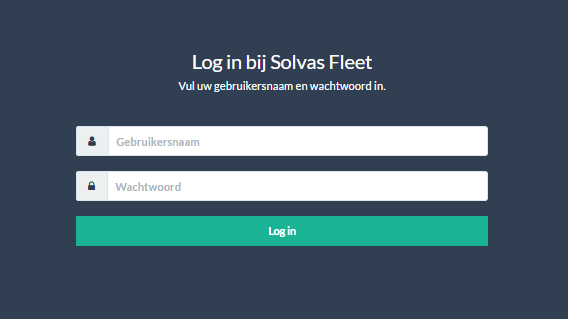
\includegraphics[width=0.6\textwidth]{img/fig1.png}
	\caption{Inlogscherm Solvas Fleet} 
	\label{fig:1} 
\end{figure}

\begin{figure}
	\centering
	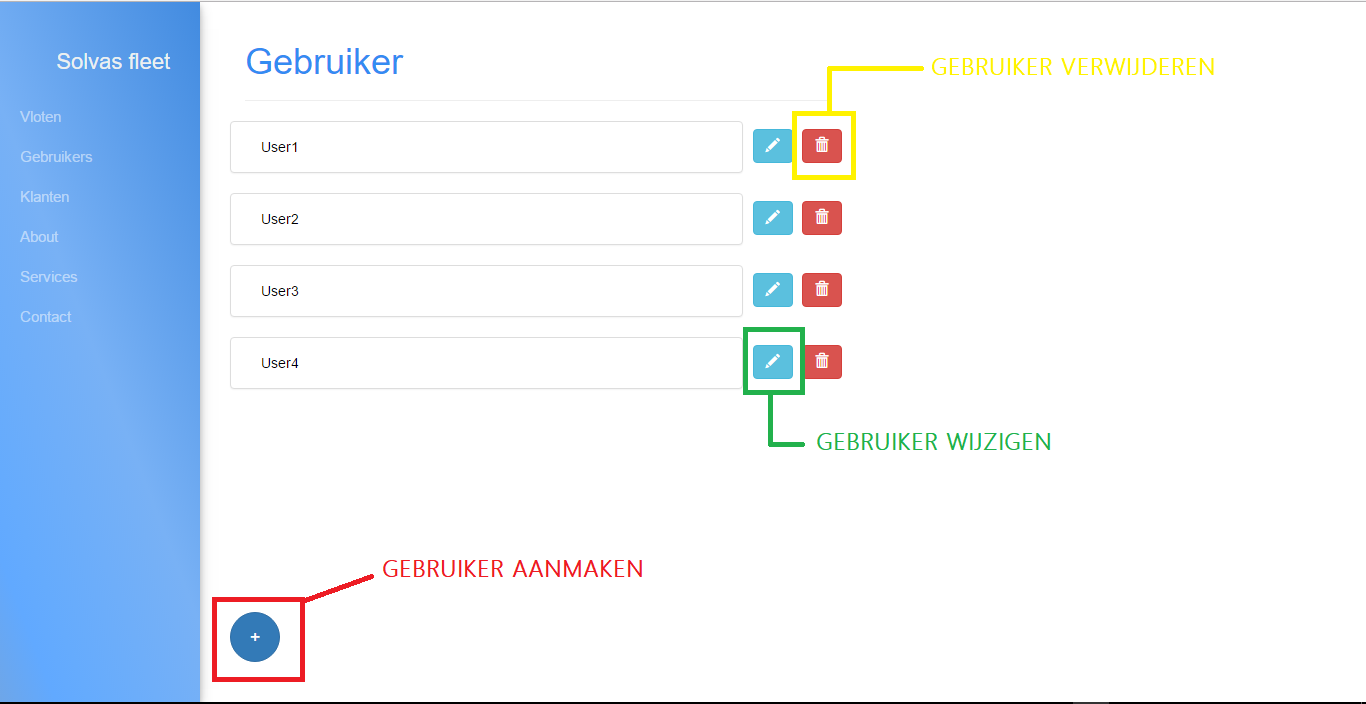
\includegraphics[width=0.9\textwidth]{img/fig2.png}
	\caption{Startscherm Solvas Fleet} 
	\label{fig:2} 
\end{figure}

\newpage
\subsection{Afmelden}
Om uit te loggen bij Solvas Fleet, volgt u onderstaande stappen:
\begin{enumerate}
	\item Rechtsboven in de bovenbalk klikt u uw naam aan.
	\item U krijgt nu een menu te zien waarin u verschillende opties ziet waaronder de optie 'Afmelden' zoals weergegeven in Figuur \ref{fig:3}.
	\item Klik vervolgens de optie 'Afmelden' aan.
	\item Tenslotte komt u opnieuw terecht bij het inlogscherm zoals weergegeven in Figuur \ref{fig:1}.
\end{enumerate}

\begin{figure}
	\centering
	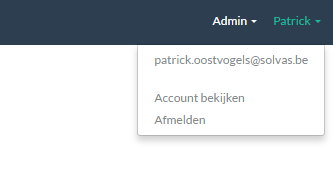
\includegraphics[width=0.5\textwidth]{img/fig3.png}
	\caption{Afmelden bij Solvas Fleet} 
	\label{fig:3} 
\end{figure}

\newpage
\section{Authorisatie}
 
\label{authorisation}
Naast authenticatie maakt de Solvas Fleet webapplicatie ook gebruik van een geautoriseerd systeem. 
Met behulp van verschillende rollen en permissies kunnen bepaalde handelingen zowel toegelaten als geweigerd worden.
Verder is het in de huidige versie van de applicatie zo dat een gebruiker op elk moment kan wisselen van actieve functie
indien deze over meerde functies beschikt (cfr. \ref{function_change}). Dit maakt het bijvoorbeeld mogelijk om als administrator voor dagelijks werk over te schakelen naar een functie met minder permissies. Zo zouden eventuele foute handelingen een minder
grote impact hebben op het systeem. Tenslotte kunnen rollen aangemaakt, bewerkt en verwijderd worden naar wens (cfr. sectie \ref{roles})
\addtocontents{toc}{\protect\newpage}
\section{Gebruik}
\subsection{Inleiding}

Zoals reeds vermeld (cfr. sectie \ref{authorisation}) beschikt elke gebruiker over \'{e}\'{e}n of meerdere functies (rollen). Aan elke van
deze functies zijn permissies gekoppeld die bepalen wat wel en niet mogelijk is onder deze functie. Om duidelijk te maken welk deel van de aangeboden functionaliteit u kan gebruiken, werd in het verdere vervolg van de handleiding elke functionaliteit gekenmerkt door een reeks van symbool. Elk symbool komt overeen met \'{e}\'{e}n van de vier standaard functies en zijn weergegeven in onderstaande tabel. 

\begin{table}[]
	\centering
	\label{table1}
	\begin{tabular}{l|l|l}
		\textbf{Functie}     & \textbf{Permissie} & Geen Permissie \\ \hline
		Admin                & \done                 & \wontfix          \\
		Productie beheerder  & \done                 & \wontfix              \\
		Verzekeringsmakelaar & \done                 & \wontfix              \\
		Klant                & \done                 & \wontfix             
	\end{tabular}
\end{table}


\newpage
\subsection{Gebruikers}
\subsubsection{Aanmaken}

\begin{todolist}
	\item[\done] Administrator
	\item[\wontfix] Productiebeheerder
	\item[\wontfix] Verzekeringsmakelaar
	\item[\wontfix] Klant 
\end{todolist}
\\
\\
Om een gebruiker aan te maken, volgt u onderstaande stappen:
\begin{enumerate}
	\item Start de Solvas Fleet applicatie en log in. U ziet het startscherm gelijkaardig zoals weergegeven in Figuur \ref{fig:2}.
	\item In de bovenbalk kiest u voor 'Gebruikers'. U ziet nu een lijst van gebruikers zoals weergegeven in Figuur \ref{fig:4}.
	\item Om een gebruiker aan te maken, klikt u de knop 'Gebruiker aanmaken' aan bovenaan de pagina. 
	\item U krijgt nu een formulier te zien zoals in Figuur \ref{fig:5} met als titel 'Gebruiker aanmaken'.
	\item Vul het formulier op een correcte manier in en bevestig het aanmaken van een gebruiker door de knop 'Gebruiker aanmaken' aan te klikken (stap 7) of annuleer het proces via de 'Annuleer' knop (stap 8) .
	\item Indien de door u ingevoerde gegevens niet correct waren, krijgt u een foutmelding te zien zoals weergegeven in Figuur \ref{fig:6}. Vul de gegevens opnieuw in en verbeter uw fouten.
	\item Indien u het aanmaken van een gebruiker bevestigt, komt u opnieuw terecht bij de lijst van gebruikers. 
	\item Indien u het aanmaken van een gebruiker annuleert, komt u opnieuw terecht bij de lijst van gebruikers.
	
\end{enumerate}
\begin{figure}
	\centering
	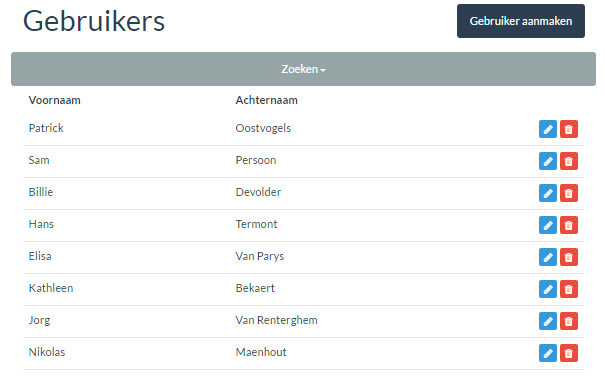
\includegraphics[width=0.8\textwidth]{img/fig4.png}
	\caption{Lijst van gebruikers} 
	\label{fig:4} 
\end{figure}


\begin{figure}
	\centering
	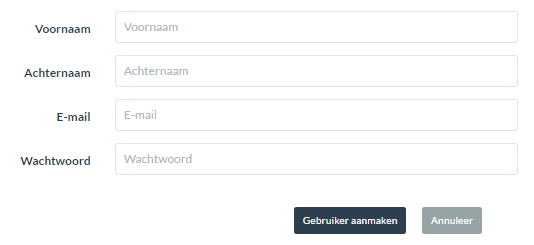
\includegraphics[width=0.5\textwidth]{img/fig5.png}
	\caption{Formulier gebruiker} 
	\label{fig:5} 
\end{figure}

\begin{figure}
	\centering
	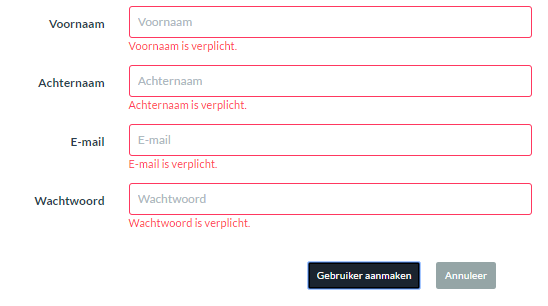
\includegraphics[width=0.5\textwidth]{img/fig6.png}
	\caption{Foutmelding gebruiker} 
	\label{fig:6} 
\end{figure}
\newpage
\subsubsection{Bekijken}

\label{user_show}
\begin{todolist}
	\item[\done] Administrator
	\item[\done] Productiebeheerder
	\item[\done] Verzekeringsmakelaar
	\item[\done] Klant 
\end{todolist}
\\
\\
Om een gebruiker te bekijken, volgt u onderstaande stappen:
\begin{enumerate}
	\item Start de Solvas Fleet applicatie en log in. U ziet het startscherm gelijkaardig zoals weergegeven in Figuur \ref{fig:2}.
	\item In de bovenbalk kiest u voor 'Gebruikers'. U ziet nu een lijst van gebruikers zoals weergegeven in Figuur \ref{fig:4}. Indien de huidige functie Klant is, klikt u rechtsboven in de bovenbalk uw naam aan. U krijgt het menu te zien als in \ref{fig:3}. Klik 'Account bekijken aan om uw informatie te bekijken'
	\item Om een gebruiker te bekijken, klikt u de desgewenste gebruiker aan.
	\item U ziet nu informatie over de gekozen gebruiker zoals weergegeven in Figuur \ref{fig:7}. 
	\item Indien u wenst terug te keren naar de lijst van gebruikers, klikt u de knop 'Terug' aan.
\end{enumerate}

\begin{figure}
	\centering
	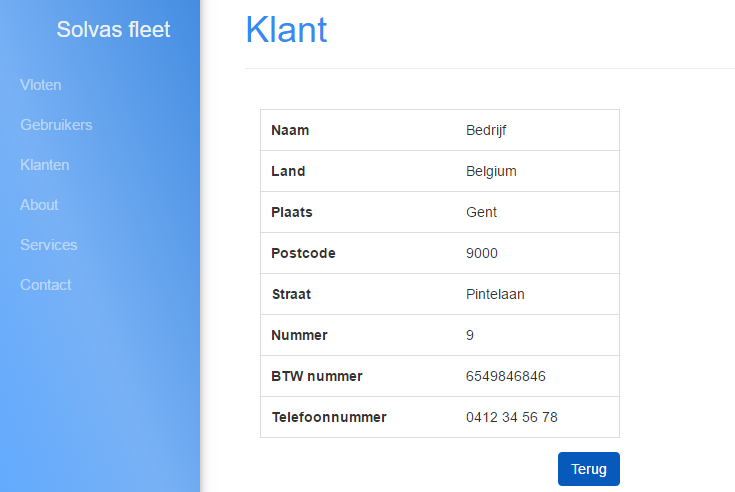
\includegraphics[width=0.7\textwidth]{img/fig7.png}
	\caption{Informatie gebruiker} 
	\label{fig:7} 
\end{figure}
\newpage
\subsubsection{Bewerken}
\begin{todolist}
	\item[\done] Administrator
	\item[\wontfix] Productiebeheerder
	\item[\wontfix] Verzekeringsmakelaar
	\item[\wontfix] Klant 
\end{todolist}
\\
\\
Om een gebruiker te bewerken, volgt u onderstaande stappen:
\begin{enumerate}
	\item Start de Solvas Fleet applicatie en log in. U ziet het startscherm gelijkaardig zoals weergegeven in Figuur \ref{fig:2}.
	\item In de bovenbalk kiest u voor 'Gebruikers'. U ziet nu een lijst van gebruikers zoals weergegeven in Figuur \ref{fig:4}.
	\item Om een gebruiker te bewerken, klikt u het lichtblauwe penseel icoon aan.
	\item U krijgt nu een formulier te zien zoals in Figuur \ref{fig:5} met als titel 'Gebruiker bewerken'.
	\item Vul het formulier op een correcte manier in en bevestig het bewerken van een gebruiker door de knop 'Gebruiker bewerken' aan te klikken (stap 7) of annuleer het proces via de 'Annuleer' knop (stap 8) .
	\item Indien de door u ingevoerde gegevens niet correct waren, krijgt u een foutmelding te zien zoals weergegeven in Figuur \ref{fig:6}. Vul de gegevens opnieuw in en verbeter uw fouten.
	\item Indien u het bewerken van een gebruiker bevestigt, komt u opnieuw terecht bij de lijst van gebruikers. 
	\item Indien u het bewerken van een gebruiker annuleert, komt u opnieuw terecht bij de lijst van gebruikers.
	
\end{enumerate}

\subsubsection{Verwijderen}
\begin{todolist}
	\item[\done] Administrator
	\item[\wontfix] Productiebeheerder
	\item[\wontfix] Verzekeringsmakelaar
	\item[\wontfix] Klant 
\end{todolist}
\\
\\
Om een gebruiker te verwijderen, volgt u onderstaande stappen:
\begin{enumerate}
	\item Start de Solvas Fleet applicatie en log in. U ziet het startscherm weergegeven in Figuur \ref{fig:2}.
	\item In de bovenbalk kiest u voor 'Gebruikers'. U ziet nu een lijst van alle gebruikers zoals weergegeven in Figuur \ref{fig:4}.
	\item Om een gebruiker te verwijderen, klikt u op het rode vuilbak icoon.
	\item De applicatie vraagt om een extra bevestiging. Indien u wilt doorgaan met het verwijderen, kiest u voor 'Ja'. In het andere geval kiest u voor 'Nee'.
	\item Het systeem verwijdert de door u gekozen gebruiker en u bevindt zich opnieuw naar de lijst van gebruikers (Figuur \ref{fig:4}).
\end{enumerate}
\subsubsection{Zoeken}
\begin{todolist}
	\item[\done] Administrator
	\item[\done] Productiebeheerder
	\item[\done] Verzekeringsmakelaar
	\item[\done] Klant 
\end{todolist}
\\
\\
Om een gebruiker te zoeken, volgt u onderstaande stappen:
\begin{enumerate}
	\item Start de Solvas Fleet applicatie en log in. U ziet het startscherm weergegeven in Figuur \ref{fig:2}.
	\item In de bovenbalk kiest u voor 'Gebruikers'. U ziet nu een lijst van alle gebruikers zoals weergegeven in Figuur \ref{fig:4}.
	\item Om een gebruiker te zoeken, klikt u de grijze balk met als tekst 'Zoeken' aan. 
	\item Vervolgens krijgt u een formulier te zien zoals weergegeven in Figuur \ref{fig:8}.
	\item Vul de velden in waarop u wilt zoeken en druk op het zoek icoon onderaan het formulier.
	\item U krijgt nu een lijst te zien zoals weergegeven in \ref{fig:4} met alle gebruikers die voldoen aan uw ingevoerde zoekopdracht.
\end{enumerate}

\begin{figure}
	\centering
	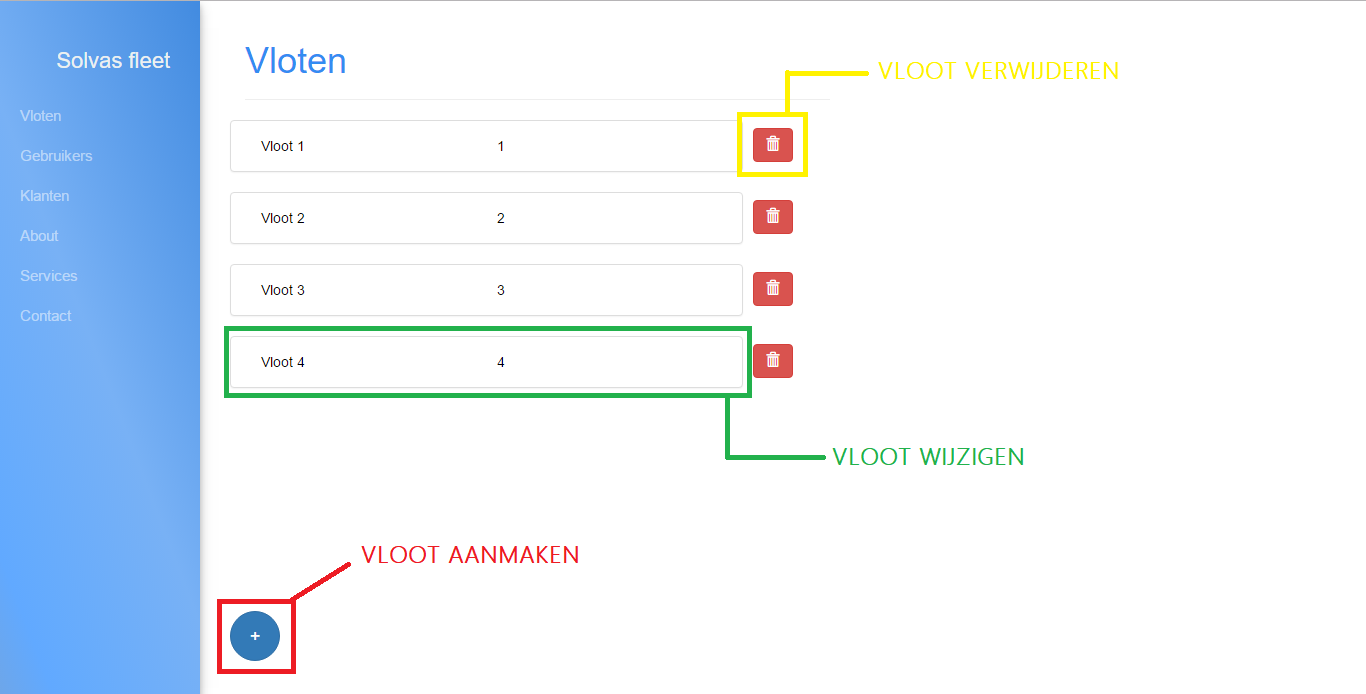
\includegraphics[width=0.5\textwidth]{img/fig8.png}
	\caption{Zoeken naar gebruiker(s)} 
	\label{fig:8} 
\end{figure}


\subsubsection{Functie toevoegen}

\begin{todolist}
	\item[\done] Administrator
	\item[\done] Productiebeheerder
	\item[\done] Verzekeringsmakelaar
	\item[\wontfix] Klant 
\end{todolist}
\\
\\
Om een functie aan een gebruiker toe te voegen, volgt u onderstaande stappen:
\begin{enumerate}
	\item Volg de stappen uit sectie \ref{user_show} tot u de informatie van de gebruiker te zien krijgt zoals weergegeven in Figuur \ref{fig:7}.
	\item Hier worden alle functies van een gebruiker weergegeven.
	\item Om een functie aan te maken, klikt u de knop 'Functie aanmaken' aan.
	\item Vervolgens krijgt u een formulier te zien zoals weergegeven in Figuur \ref{fig:9} met als titel 'Functie aanmaken'.
	\item Vul de velden op een correcte manier in en bevestig of annuleer het aanmaken van een functie.
	\item U komt opnieuw terecht op de informatiepagina van de gebruiker zoals weergegeven in Figuur \ref{fig:7}.
\end{enumerate}

\begin{figure}
	\centering
	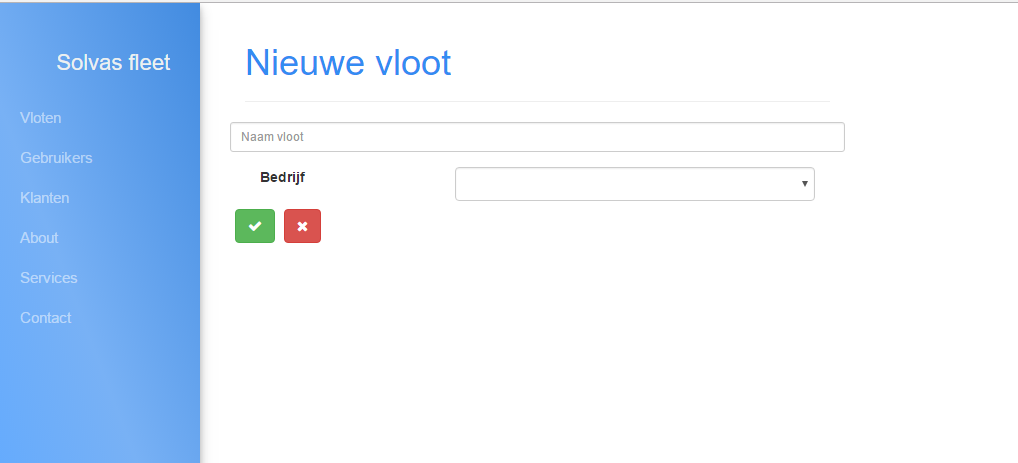
\includegraphics[width=0.5\textwidth]{img/fig9.png}
	\caption{Formulier functie} 
	\label{fig:9} 
\end{figure}



\subsubsection{Functie verwijderen}
\begin{todolist}
	\item[\done] Administrator
	\item[\wontfix] Productiebeheerder
	\item[\wontfix] Verzekeringsmakelaar
	\item[\wontfix] Klant 
\end{todolist}
\\
\\
Om een functie van een gebruiker te verwijderen, volgt u onderstaande stappen:
\begin{enumerate}
	\item Volg de stappen uit sectie \ref{user_show} tot u de informatie van de gebruiker te zien krijgt zoals weergegeven in Figuur \ref{fig:7}.
	\item Hier worden alle functies van een gebruiker weergegeven.
	\item Om een functie te verwijderen, klikt u op het rode vuilbak icoon.
	\item De applicatie vraagt om een extra bevestiging. Indien u wilt doorgaan met het verwijderen, kiest u voor 'Ja'. In het andere geval kiest u voor 'Nee'.
	\item Het systeem verwijdert de door u gekozen functie van de gebruiker.
\end{enumerate}



\subsubsection{Actieve functie wijzigen}

\label{function_change}
\begin{todolist}
	\item[\done] Administrator
	\item[\done] Productiebeheerder
	\item[\done] Verzekeringsmakelaar
	\item[\done] Klant 
\end{todolist}
\\
\\
Om de actieve functie van een gebruiker te wijzigen, volgt u onderstaande stappen:
\begin{enumerate}
	\item Rechtsboven in de bovenbalk klikt u uw actieve functie aan.
	\item U krijgt nu een menu te zien waarin u al uw beschikbare functies ziet zoals weergegeven in Figuur \ref{fig:10}.
	\item Wijzig de actieve functie door een nieuwe functie aan te klikken.
	\item Het systeem verandert onmiddelijk de hele applicatie volgens de door u gekozen functie.
\end{enumerate}

\begin{figure}
	\centering
	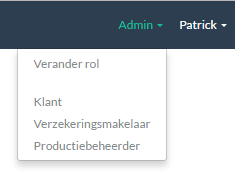
\includegraphics[width=0.5\textwidth]{img/fig10.png}
	\caption{Actieve functie wijzigen} 
	\label{fig:10} 
\end{figure}

\newpage
\subsubsection{Taal kiezen}
\begin{todolist}
	\item[\done] Administrator
	\item[\done] Productiebeheerder
	\item[\done] Verzekeringsmakelaar
	\item[\done] Klant 
\end{todolist}
\\
\\
De webapplicatie ondersteunt het gebruik van verschillende talen. 
De huidige versie van de webapplicatie ondersteunt zowel Nederlands als Engels. 
Om een taal naar keuze in te stellen, dient u volgende stappen te ondernemen::
\begin{enumerate}
	\item Volg de stappen uit sectie \ref{user_show} tot u de informatie van de gebruiker te zien krijgt zoals weergegeven in Figuur \ref{fig:7}.
	\item Om uw taal naar keuze in te stellen, kiest uw de gewenste taal uit de taal optie zoals weergegeven in Figuur \ref{fig:7}
	\item Het systeem verandert onmiddelijk de hele applicatie volgens de door u gekozen taal.
\end{enumerate}

\newpage
\subsection{Rollen}
\label{roles}
\subsubsection{Aanmaken}

\begin{todolist}
	\item[\done] Administrator
	\item[\wontfix] Productiebeheerder
	\item[\wontfix] Verzekeringsmakelaar
	\item[\wontfix] Klant 
\end{todolist}
\\
\\
Om een rol aan te maken, volgt u onderstaande stappen:
\begin{enumerate}
	\item Start de Solvas Fleet applicatie en log in. U ziet het startscherm gelijkaardig zoals weergegeven in Figuur \ref{fig:2}.
	\item In de bovenbalk kiest u voor 'Gebruikers' en dan voor 'Rollen'. U ziet nu een lijst van rollen zoals weergegeven in Figuur \ref{fig:11}.
	\item Om een rol aan te maken, klikt u de knop 'Rol aanmaken' aan bovenaan de pagina. 
	\item U krijgt nu een formulier te zien zoals in Figuur \ref{fig:12} met als titel 'Rol aanmaken'.
	\item Vul een naam in voor de rol en kies voor elk onderdeel van de applicatie de juiste permissie die aan de rol zal toegekend worden.
	\item Bevestig of annuleer het aanmaken van de rol door de knop 'Rol aanmaken' of 'Annuleer' aan te klikken.
	\item Indien de door u ingevoerde gegevens niet correct waren, krijgt u een foutmelding te zien.
	\item U komt opnieuw terecht bij de lijst van rollen.
	
\end{enumerate}
\begin{figure}
	\centering
	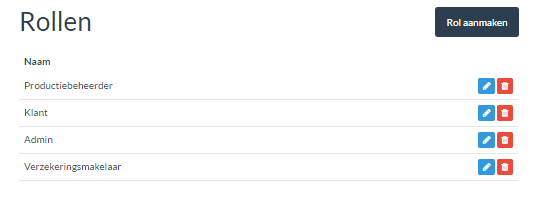
\includegraphics[width=0.8\textwidth]{img/fig11.png}
	\caption{Lijst van rollen} 
	\label{fig:11} 
\end{figure}

\begin{figure}
	\centering
	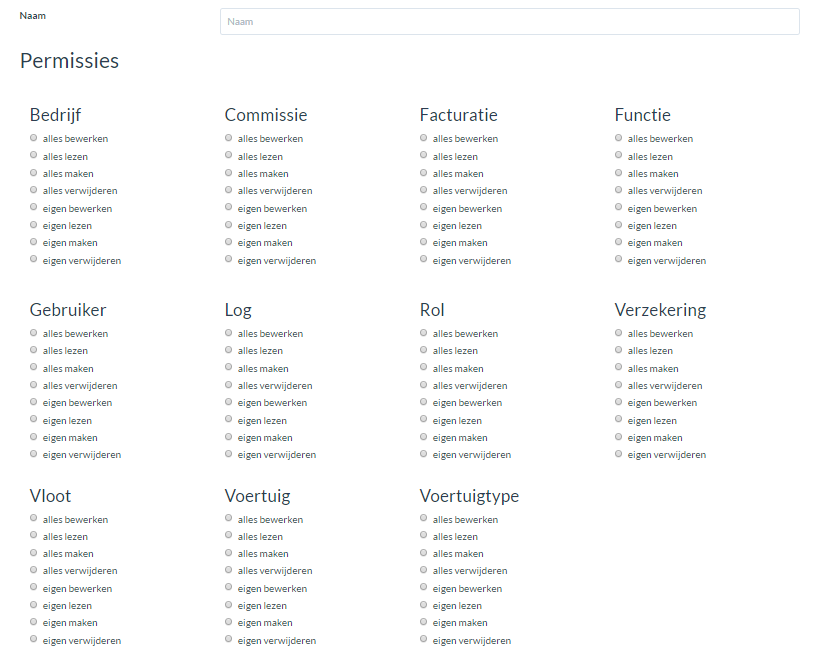
\includegraphics[width=0.8\textwidth]{img/fig12.png}
	\caption{Formulier rol} 
	\label{fig:12} 
\end{figure}
\newpage
\subsubsection{Bekijken}
\begin{todolist}
	\item[\done] Administrator
	\item[\done] Productiebeheerder
	\item[\done] Verzekeringsmakelaar
	\item[\done] Klant 
\end{todolist}
\\
\\
Om een rol te bekijken, volgt u onderstaande stappen:
\begin{enumerate}
	\item Start de Solvas Fleet applicatie en log in. U ziet het startscherm gelijkaardig zoals weergegeven in Figuur \ref{fig:2}.
	\item In de bovenbalk kiest u voor 'Gebruikers' en dan voor 'Rollen'. U ziet nu een lijst van rollen zoals weergegeven in Figuur \ref{fig:11}.
	\item Om een rol te bekijken, klikt u de desgewenste rol aan.
	\item U ziet nu informatie over de gekozen rol en zijn permissies zoals weergegeven in Figuur \ref{fig:12}. 
	\item Indien u wenst terug te keren naar de lijst van rollen, klikt u de knop 'Terug' aan.
\end{enumerate}

\newpage
\subsubsection{Bewerken}
\begin{todolist}
	\item[\done] Administrator
	\item[\wontfix] Productiebeheerder
	\item[\wontfix] Verzekeringsmakelaar
	\item[\wontfix] Klant 
\end{todolist}
\\
\\
Om een rol te bewerken, volgt u onderstaande stappen:
\begin{enumerate}
	\item Start de Solvas Fleet applicatie en log in. U ziet het startscherm gelijkaardig zoals weergegeven in Figuur \ref{fig:2}.
	\item In de bovenbalk kiest u voor 'Gebruikers' en dan voor 'Rollen'. U ziet nu een lijst van rollen zoals weergegeven in Figuur \ref{fig:11}.
	\item Om een rol te bewerken, klikt u het lichtblauwe penseel icoon aan. 
	\item U krijgt nu een formulier te zien zoals in Figuur \ref{fig:12} met als titel 'Rol bewerken' en alle permissies van de rol.
	\item Vul het formulier op een correcte manier in en bevestig het bewerken van een rol door de knop 'Rol bewerken' aan te klikken of annuleer het proces via de 'Annuleer' knop.
	\item Indien de door u ingevoerde gegevens niet correct waren, krijgt u een foutmelding te zien.
	
	
\end{enumerate}
\subsubsection{Verwijderen}

\begin{todolist}
	\item[\done] Administrator
	\item[\wontfix] Productiebeheerder
	\item[\wontfix] Verzekeringsmakelaar
	\item[\wontfix] Klant 
\end{todolist}
\\
\\
Om een rol te verwijderen, volgt u onderstaande stappen:
\begin{enumerate}
	\item Start de Solvas Fleet applicatie en log in. U ziet het startscherm weergegeven in Figuur \ref{fig:2}.
	\item In de bovenbalk kiest u voor 'Gebruikers' en dan voor 'Rollen'. U ziet nu een lijst van alle rollen zoals weergegeven in Figuur \ref{fig:11}.
	\item Om een rol te verwijderen, klikt u op het rode vuilbak icoon. 
	\item De applicatie vraagt om een extra bevestiging. Indien u wilt doorgaan met het verwijderen, kiest u voor 'Ja'. In het andere geval kiest u voor 'Nee'.
	\item Het systeem verwijdert de door u gekozen rol en u bevindt zich opnieuw naar de lijst van rollen (Figuur \ref{fig:11}).
\end{enumerate}
\newpage
\subsection{Bedrijven}
\subsubsection{Aanmaken}
\label{company_new}
\begin{todolist}
	\item[\done] Administrator
	\item[\done] Productiebeheerder
	\item[\done] Verzekeringsmakelaar
	\item[\wontfix] Klant 
\end{todolist}
\\
\\
Om een bedrijf aan te maken, volgt u onderstaande stappen:
\begin{enumerate}
	\item Start de Solvas Fleet applicatie en log in. U ziet het startscherm gelijkaardig zoals weergegeven in Figuur \ref{fig:2}.
	\item In de bovenbalk kiest u voor 'Bedrijven'. U ziet nu een lijst van bedrijven zoals weergegeven in Figuur \ref{fig:13}.
	\item Om een bedrijf aan te maken, klikt u de knop 'Bedrijf aanmaken' aan bovenaan de pagina. 
	\item U krijgt nu een formulier te zien zoals in Figuur \ref{fig:14} met als titel 'Bedrijf aanmaken'.
	\item Vul het formulier op een correcte manier in en bevestig het aanmaken van een bedrijf door de knop 'Bedrijf aanmaken' aan te klikken (stap 7) of annuleer het proces via de 'Annuleer' knop (stap 8) .
	\item Indien de door u ingevoerde gegevens niet correct waren, krijgt u een gelijkaardige foutmelding te zien zoals weergegeven in Figuur \ref{fig:6}. Vul de gegevens opnieuw in en verbeter uw fouten.
	\item Indien u het aanmaken van een bedrijf bevestigt, komt u opnieuw terecht bij de lijst van bedrijven. 
	\item Indien u het aanmaken van een bedrijf annuleert, komt u opnieuw terecht bij de lijst van bedrijven.
	
\end{enumerate}
\begin{figure}
	\centering
	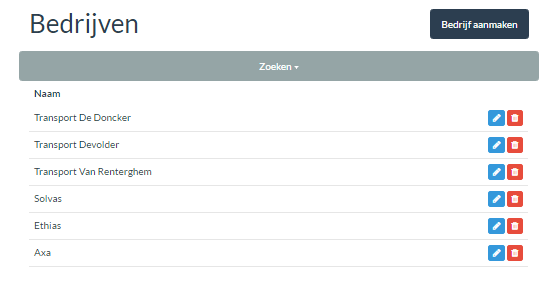
\includegraphics[width=0.8\textwidth]{img/fig13.png}
	\caption{Lijst van bedrijven} 
	\label{fig:13} 
\end{figure}

\begin{figure}
	\centering
	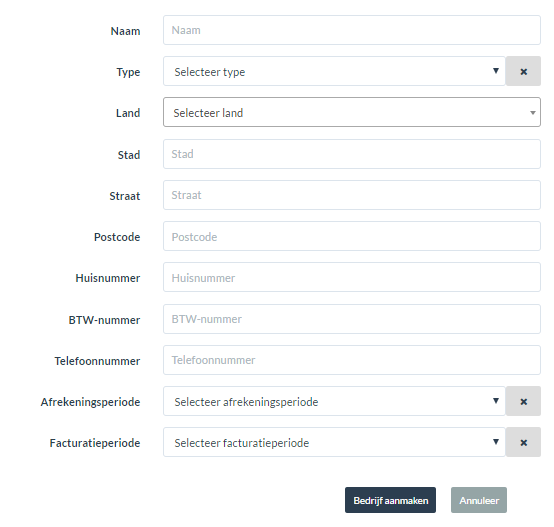
\includegraphics[width=0.8\textwidth]{img/fig14.png}
	\caption{Formulier bedrijf} 
	\label{fig:14} 
\end{figure}


\subsubsection{Bekijken}
\label{company_show}
\begin{todolist}
	\item[\done] Administrator
	\item[\done] Productiebeheerder
	\item[\done] Verzekeringsmakelaar
	\item[\done] Klant 
\end{todolist}
\\
\\
Om een bedrijf te bekijken, volgt u onderstaande stappen:
\begin{enumerate}
	\item Start de Solvas Fleet applicatie en log in. U ziet het startscherm gelijkaardig zoals weergegeven in Figuur \ref{fig:2}.
	\item In de bovenbalk kiest u voor 'Bedrijven'. U ziet nu een lijst van bedrijven zoals weergegeven in Figuur \ref{fig:13}. Indien de huidige functie Klant is, klikt u lichtsboven in de bovenbalk op het solvas fleet logo om de gegevens van uw bedrijf te kunnen bekijken.
	\item Om een bedrijf te bekijken, klikt u het desgewenste bedrijf aan	. 
	\item U ziet nu informatie over het gekozen bedrijf. Deze informatie is afhankelijk van het bedrijfstype.
	\begin{enumerate}
		\item Voor een klant ziet u de informatie zoals weergegeven in Figuur \ref{fig:15}.
		Naast de algemene informatie zie u ook alle vloten en verzekeringscontracten van het bedrijf en kan u hier bewerkingen op uit voeren (afhankelijk van functie). Voor verdere informatie cfr. sectie \ref{fleets} en sectie \ref{insurances}.
		\item Voor een verzekeringsbedrijf ziet u de informatie zoals weergegeven in Figuur \ref{fig:16}.
		Naast de algemene informatie zie u ook alle verzekeringswaarborgen en verzekeringscontracten van het bedrijf en kan u hier bewerkingen op uit voeren (afhankelijk van functie). Voor verdere informatie cfr. sectie \ref{sureties} en sectie \ref{insurances}.
	\end{enumerate} 
	\item Indien u wenst terug te keren naar de lijst van bedrijven, klikt u de knop 'Terug' aan.
\end{enumerate}

\begin{figure}
	\centering
	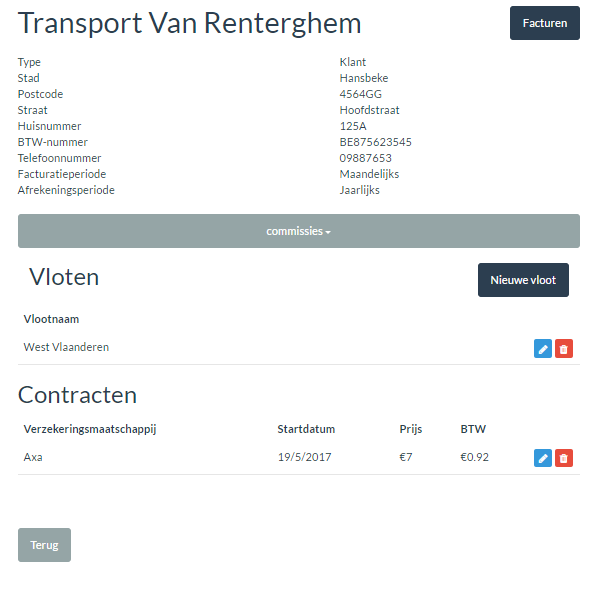
\includegraphics[width=0.6\textwidth]{img/fig15.png}
	\caption{Informatie klant} 
	\label{fig:15} 
\end{figure}

\begin{figure}
	\centering
	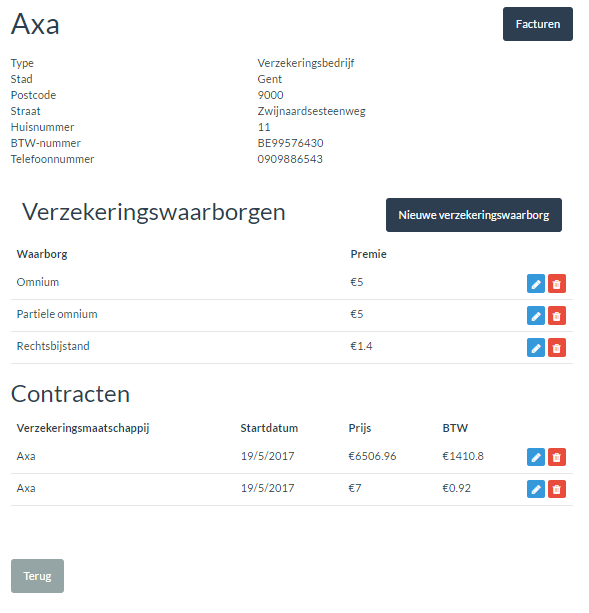
\includegraphics[width=0.6\textwidth]{img/fig16.png}
	\caption{Informatie verzekeringsbedrijf} 
	\label{fig:16} 
\end{figure}



\subsubsection{Bewerken}
\label{company_edit}
\begin{todolist}
	\item[\done] Administrator
	\item[\done] Productiebeheerder
	\item[\done] Verzekeringsmakelaar
	\item[\wontfix] Klant 
\end{todolist}
\\
\\
Om een bedrijf te bewerken, volgt u onderstaande stappen:
\begin{enumerate}
	\item Start de Solvas Fleet applicatie en log in. U ziet het startscherm gelijkaardig zoals weergegeven in Figuur \ref{fig:2}.
	\item In de bovenbalk kiest u voor 'Bedrijven'. U ziet nu een lijst van bedrijven zoals weergegeven in Figuur \ref{fig:13}.
	\item Om een gebruiker te bewerken, klikt u het lichtblauwe penseel icoon aan.
	\item U krijgt nu een formulier te zien zoals in Figuur \ref{fig:14} met als titel 'Bedrijf bewerken'.
	\item Vul het formulier op een correcte manier in en bevestig het bewerken van een bedrijf door de knop 'Bedrijf bewerken' aan te klikken (stap 7) of annuleer het proces via de 'Annuleer' knop (stap 8) .
	\item Indien de door u ingevoerde gegevens niet correct waren, krijgt u een gelijkaardige foutmelding te zien zoals weergegeven in Figuur \ref{fig:6}. Vul de gegevens opnieuw in en verbeter uw fouten.
	\item Indien u het bewerken van een bedrijf bevestigt, komt u opnieuw terecht bij de lijst van bedrijven. 
	\item Indien u het bewerken van een bedrijf annuleert, komt u opnieuw terecht bij de lijst van bedrijven.
	
\end{enumerate}

\subsubsection{Verwijderen}
\begin{todolist}
	\item[\done] Administrator
	\item[\done] Productiebeheerder
	\item[\done] Verzekeringsmakelaar
	\item[\wontfix] Klant 
\end{todolist}
\\
\\
Om een bedrijf te verwijderen, volgt u onderstaande stappen:
\begin{enumerate}
	\item Start de Solvas Fleet applicatie en log in. U ziet het startscherm weergegeven in Figuur \ref{fig:2}.
	\item In de bovenbalk kiest u voor 'Bedrijven'. U ziet nu een lijst van alle bedrijven zoals weergegeven in Figuur \ref{fig:13}.
	\item Om een bedrijf te verwijderen, klikt u op het rode vuilbak icoon. 
	\item De applicatie vraagt om een extra bevestiging. Indien u wilt doorgaan met het verwijderen, kiest u voor 'Ja'. In het andere geval kiest u voor 'Nee'.
	\item Het systeem verwijdert het door u gekozen bedrijf en u bevindt zich opnieuw naar de lijst van bedrijven (Figuur \ref{fig:13}).
\end{enumerate}

\subsubsection{Zoeken}
\begin{todolist}
	\item[\done] Administrator
	\item[\done] Productiebeheerder
	\item[\done] Verzekeringsmakelaar
	\item[\done] Klant 
\end{todolist}
\\
\\
Om een bedrijf te zoeken, volgt u onderstaande stappen:
\begin{enumerate}
	\item Start de Solvas Fleet applicatie en log in. U ziet het startscherm weergegeven in Figuur \ref{fig:2}.
	\item In de bovenbalk kiest u voor 'Bedrijven'. U ziet nu een lijst van alle bedrijven zoals weergegeven in Figuur \ref{fig:13}.
	\item Om een gebruiker te zoeken, klikt u de grijze balk met als tekst 'Zoeken' aan.
	\item Vervolgens krijgt u een formulier te zien zoals weergegeven in Figuur \ref{fig:17}.
	\item Vul de velden in waarop u wilt zoeken en druk op het zoek icoon onderaan het formulier.
	\item U krijgt nu een lijst te zien zoals weergegeven in \ref{fig:13} met alle bedrijven die voldoen aan uw ingevoerde zoekopdracht.
\end{enumerate}


\begin{figure}
	\centering
	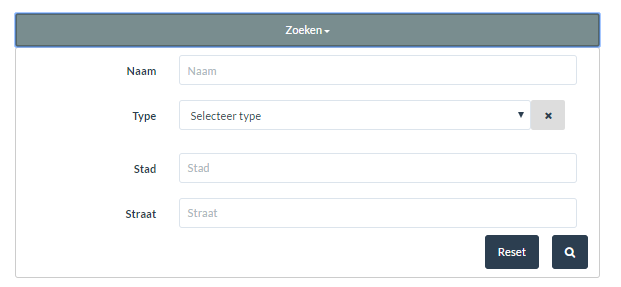
\includegraphics[width=0.5\textwidth]{img/fig17.png}
	\caption{Zoeken naar bedrijf/bedrijven} 
	\label{fig:17} 
\end{figure}

\subsubsection{Commissie wijzigen}
\label{company_commision}
\begin{todolist}
	\item[\done] Administrator
	\item[\done] Productiebeheerder
	\item[\done] Verzekeringsmakelaar
	\item[\wontfix] Klant 
\end{todolist}
\\
\\
\textbf{Dit is enkel van toepassing voor bedrijven die als klant geregistreerd zijn.}
\\
Om de commisies op een bedrijf te wijzigen, volgt u onderstaande stappen:
\begin{enumerate}
		\item Volg de stappen uit sectie \ref{company_show} tot u de informatie van het bedrijf te zien krijgt zoals weergegeven in Figuur \ref{fig:15}.
	\item Om de commissies te wijzigen, klikt u de grijze balk met als tekst 'commissies' aan.
	\item Hierop krijgt u de huidige commissiewaarden terug. Indien u deze waarden wil wijzigen dient u
	de knop 'Wijzig' aan te zetten weergegeven zoals in Figuur \ref{fig18}.
	\item Vervolgens krijgt u een formulier te zien zoals weergegeven in Figuur \ref{fig:18}.
	\item Vul het formulier op een correcte manier in en bevestig het bewerken van de commissies op een bedrijf door de knop 'Commissie bewerken' te klikken of annuleer het proces via de 'Annuleer' knop.
	\item Indien de door u ingevoerde gegevens niet correct waren, krijgt u een gelijkaardige foutmelding te zien zoals weergegeven in Figuur \ref{fig:6}. Vul de gegevens opnieuw in en verbeter uw fouten.
\end{enumerate}


\begin{figure}
	\centering
	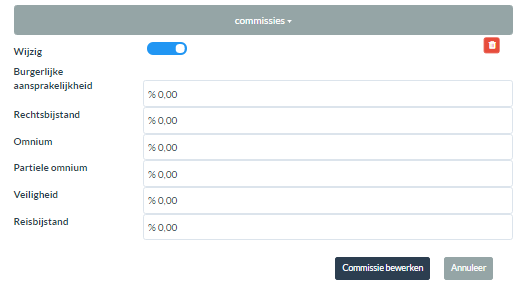
\includegraphics[width=0.5\textwidth]{img/fig47.png}
	\caption{Lijst van commissiewaarden} 
	\label{fig:18} 
\end{figure}



\subsubsection{Facturen bekijken}

\label{company_invoice_show}
 \begin{todolist}
 	\item[\done] Administrator
 	\item[\done] Productiebeheerder
 	\item[\done] Verzekeringsmakelaar
 	\item[\done] Klant 
 \end{todolist}
 \\
 \\
 Om de facturen van een bedrijf te bekijken, volgt u onderstaande stappen:
 \begin{enumerate}
 	\item Volg de stappen uit sectie \ref{company_show} tot u de informatie van het bedrijf te zien krijgt zoals weergegeven in Figuur \ref{fig:15} of Figuur \ref{fig:16}.
 	\item Om de facturen te bekijken, klikt u de knop 'Facturen' aan bovenaan de pagina.
 	\item Hierop krijgt u een lijst van alle facturen van het bedrijf terug weergegeven zoals in Figuur \ref{fig:19}.
 	\item Indien u wenst terug te keren naar de informatie van het bedrijf, klikt u de knop 'Terug' aan.
 \end{enumerate}

\begin{figure}
	\centering
	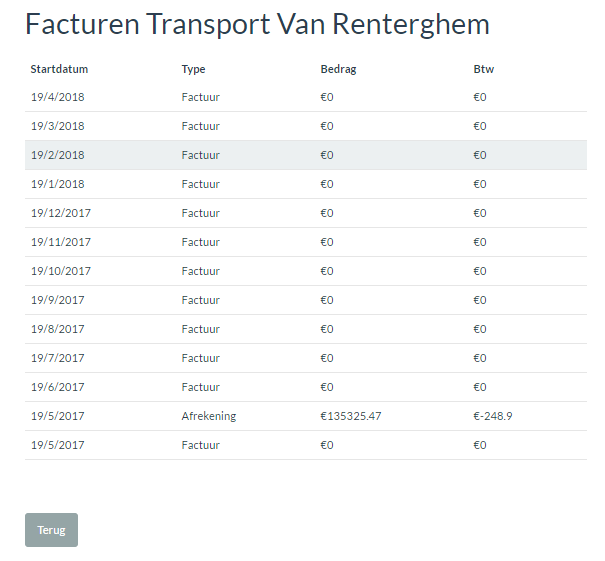
\includegraphics[width=0.5\textwidth]{img/fig19.png}
	\caption{Lijst van facturen} 
	\label{fig:19} 
\end{figure}
\newpage
\subsection{Vloten}
\label{fleets}
\subsubsection{Aanmaken}

\begin{todolist}
	\item[\done] Administrator
	\item[\done] Productiebeheerder
	\item[\done] Verzekeringsmakelaar
	\item[\wontfix] Klant 
\end{todolist}
\\
\\
Om een vloot aan te maken, volgt u onderstaande stappen:
\begin{enumerate}
	\item Start de Solvas Fleet applicatie en log in. U ziet het startscherm gelijkaardig zoals weergegeven in Figuur \ref{fig:2}.
	\item In de bovenbalk kiest u voor 'Bedrijven' en dan voor 'Vloten'. U ziet nu een lijst van vloten zoals weergegeven in Figuur \ref{fig:20}.
	\item Om een vloot aan te maken, klikt u de knop 'Vloot aanmaken' aan bovenaan de pagina.
	\item U krijgt nu een formulier te zien zoals in Figuur \ref{fig:21} met als titel 'Vloot aanmaken'.
	\item Vul het formulier op een correcte manier in en bevestig het aanmaken van een vloot door de knop 'Vloot aanmaken' aan te klikken (stap 7) of annuleer het proces via de 'Annuleer' knop (stap 8) .
	\item Indien de door u ingevoerde gegevens niet correct waren, krijgt u een gelijkaardige foutmelding te zien zoals weergegeven in Figuur \ref{fig:6}. Vul de gegevens opnieuw in en verbeter uw fouten.
	\item Indien u het aanmaken van een vloot bevestigt, komt u opnieuw terecht bij de lijst van vloten. 
	
	\item Indien u het aanmaken van een vloot annuleert, komt u opnieuw terecht bij de lijst van vloten.
	
\end{enumerate}
\begin{figure}
	\centering
	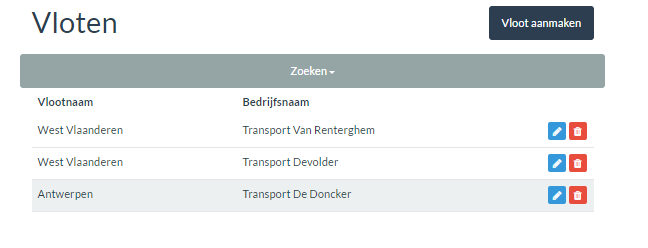
\includegraphics[width=0.8\textwidth]{img/fig20.png}
	\caption{Lijst van vloten} 
	\label{fig:20} 
\end{figure}


\begin{figure}
	\centering
	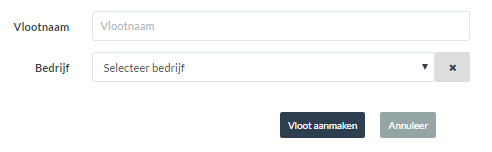
\includegraphics[width=0.5\textwidth]{img/fig21.png}
	\caption{Formulier vloot} 
	\label{fig:21} 
\end{figure}


\newpage
\subsubsection{Bekijken}
\label{fleet_show}
\begin{todolist}
	\item[\done] Administrator
	\item[\done] Productiebeheerder
	\item[\done] Verzekeringsmakelaar
	\item[\done] Klant 
\end{todolist}
\\
\\
Om een vloot te bekijken, volgt u onderstaande stappen:
\begin{enumerate}
	\item Start de Solvas Fleet applicatie en log in. U ziet het startscherm gelijkaardig zoals weergegeven in Figuur \ref{fig:2}.
	\item In de bovenbalk kiest u voor 'Bedrijven' en dan voor 'Vloten'. U ziet nu een lijst van vloten zoals weergegeven in Figuur \ref{fig:20}. Indien de huidige functie Klant is, kiest u in de bovenbalk voor 'Vloten' waarna u een lijst van al uw vloten krijgt te zien.
	\item Om een vloot te bekijken, klikt u de desgewenste vloot aan	. 
	\item U ziet nu informatie over de gekozen vloot zoals weergegeven in Figuur \ref{fig:22}. 
	\item Indien u wenst terug te keren naar de lijst van vloten, klikt u de knop 'Terug' aan.
\end{enumerate}

\begin{figure}
	\centering
	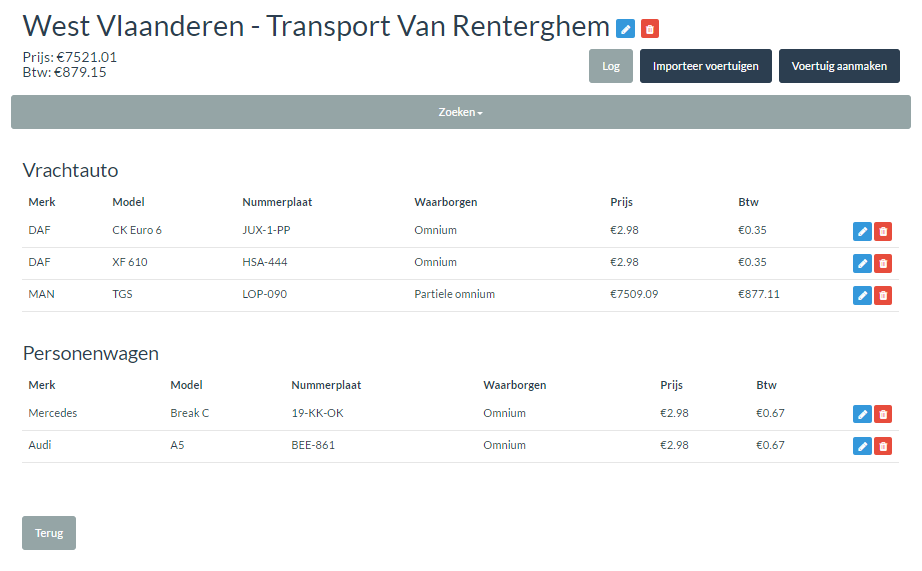
\includegraphics[width=0.8\textwidth]{img/fig22.png}
	\caption{Informatie vloot} 
	\label{fig:22} 
\end{figure}
\newpage
\subsubsection{Bewerken}
\begin{todolist}
	\item[\done] Administrator
	\item[\done] Productiebeheerder
	\item[\done] Verzekeringsmakelaar
	\item[\wontfix] Klant 
\end{todolist}
\\
\\
Om een vloot te bewerken, volgt u onderstaande stappen:
\begin{enumerate}
	\item Start de Solvas Fleet applicatie en log in. U ziet het startscherm gelijkaardig zoals weergegeven in Figuur \ref{fig:2}.
	\item In de bovenbalk kiest u voor 'Bedrijven' en dan voor 'Vloten'. U ziet nu een lijst van vloten zoals weergegeven in Figuur \ref{fig:20}.
	\item Om een vloot te bewerken, klikt u het lichtblauwe penseel icoon aan. 
	\item U krijgt nu een formulier te zien zoals in Figuur \ref{fig:21} met als titel 'Vloot bewerken'.
	\item Vul het formulier op een correcte manier in en bevestig het bewerken van een vloot door de knop 'Vloot bewerken' aan te klikken (stap 7) of annuleer het proces via de 'Annuleer' knop (stap 8) .
	\item Indien de door u ingevoerde gegevens niet correct waren, krijgt u een gelijkaardige foutmelding te zien zoals weergegeven in Figuur \ref{fig:6}. Vul de gegevens opnieuw in en verbeter uw fouten.
	\item Indien u het bewerken van een vloot bevestigt, komt u opnieuw terecht bij de lijst van vloten. 
	\item Indien u het bewerken van een vlooot annuleert, komt u opnieuw terecht bij de lijst van vloten.
	
\end{enumerate}

\subsubsection{Verwijderen}
\begin{todolist}
	\item[\done] Administrator
	\item[\done] Productiebeheerder
	\item[\done] Verzekeringsmakelaar
	\item[\wontfix] Klant 
\end{todolist}
\\
\\
\textbf{Het verwijderen van een vloot wordt enkel toegestaan indien deze vloot geen voertuigen meer bevat! Voor verdere informatie over het verwijderen van een voertuig cfr. sectie \ref{vehicles}}
\\
\\
Om een vloot te verwijderen, volgt u onderstaande stappen:
\begin{enumerate}
	\item Start de Solvas Fleet applicatie en log in. U ziet het startscherm weergegeven in Figuur \ref{fig:2}.
	\item In de bovenbalk kiest u voor 'Bedrijven' en dan voor 'Vloten'. U ziet nu een lijst van alle vloten zoals weergegeven in Figuur \ref{fig:20}.
	\item Om een vloot te verwijderen, klikt u op het rode vuilbak icoon. 
	\item De applicatie vraagt om een extra bevestiging. Indien u wilt doorgaan met het verwijderen, kiest u voor 'Ja'. In het andere geval kiest u voor 'Nee'.
	\item Het systeem verwijdert de door u gekozen vloot en u bevindt zich opnieuw naar de lijst van vloten (Figuur \ref{fig:20}).
\end{enumerate}
\subsubsection{Zoeken}
\begin{todolist}
	\item[\done] Administrator
	\item[\done] Productiebeheerder
	\item[\done] Verzekeringsmakelaar
	\item[\done] Klant 
\end{todolist}
\\
\\
Om een vloot te zoeken, volgt u onderstaande stappen:
\begin{enumerate}
	\item Start de Solvas Fleet applicatie en log in. U ziet het startscherm weergegeven in Figuur \ref{fig:2}.
\item In de bovenbalk kiest u voor 'Bedrijven' en dan voor 'Vloten'. U ziet nu een lijst van alle vloten zoals weergegeven in Figuur \ref{fig:20}.
	\item Om een vloot te zoeken, klikt u de grijze balk met als tekst 'Zoeken' aan. 
	\item Vervolgens krijgt u een formulier te zien zoals weergegeven in Figuur \ref{fig:23}.
	\item Vul de velden in waarop u wilt zoeken en druk op het zoek icoon onderaan het formulier.
	\item U krijgt nu een lijst te zien zoals weergegeven in \ref{fig:20} met alle vloten die voldoen aan uw ingevoerde zoekopdracht.
\end{enumerate}

\begin{figure}
	\centering
	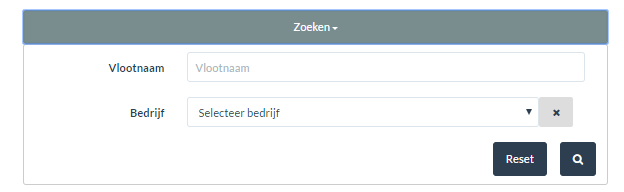
\includegraphics[width=0.5\textwidth]{img/fig23.png}
	\caption{Zoeken naar vloot/vloten} 
	\label{fig:23} 
\end{figure}

\subsubsection{Logs bekijken}

\begin{todolist}
	\item[\done] Administrator
	\item[\done] Productiebeheerder
	\item[\done] Verzekeringsmakelaar
	\item[\wontfix] Klant 
\end{todolist}
\\
\\
Om de logs van een vloot te bekijken, volgt u onderstaande stappen:
\begin{enumerate}
	\item  Volg de stappen uit sectie \ref{fleet_show} tot u de informatie van de vloot te zien krijgt zoals weergegeven in Figuur \ref{fig:22}.
	\item Om de logs te bekijken, klikt u bovenaan de knop 'Log' aan.
	\item U krijgt een lijst van logs te zien van de bewerkingen op deze vloot en al zijn voertuigen zoals weergegeven in Figuur \ref{fig:24}
	\item Indien u wenst terug te keren naar de informatiepagina van de vloot, klikt u de knop 'Terug' aan.
\end{enumerate}

\begin{figure}
	\centering
	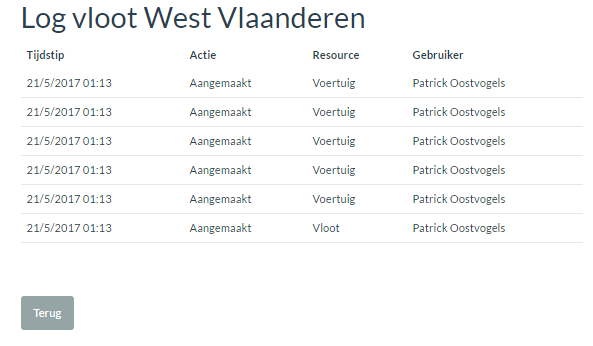
\includegraphics[width=0.5\textwidth]{img/fig24.png}
	\caption{Lijst van logs} 
	\label{fig:24} 
\end{figure}

\subsubsection{Voertuigen importeren}
\begin{todolist}
	\item[\done] Administrator
	\item[\done] Productiebeheerder
	\item[\done] Verzekeringsmakelaar
	\item[\wontfix] Klant 
\end{todolist}
\\
\\
Om een lijst van voertuigen in een vloot te importeren, volgt u onderstaande stappen:
\begin{enumerate}
	\item  Volg de stappen uit sectie \ref{fleet_show} tot u de informatie van de vloot te zien krijgt zoals weergegeven in Figuur \ref{fig:22}.
	\item Om een lijst van voertuigen te importeren, klikt u de knop 'Importeer voertuigen' aan.
	\item U krijgt een pagina te zien zoals weergeven in Figuur \ref{fig:25}
	\item Het importeren van een lijst van voertuigen moet voldoen aan een vastgelegd formaat. Indien u niet weet hoe dit formaat eruit ziet, is er een voorbeeldbestand voorzien. Om dit bestand te verkrijgen, klikt u de knop 'Download voorbeeld bestand' aan.
	\item Indien u over een lijst van voertuigen in het juiste formaat beschikt, kan u de lijst uploaden door de knop 'Bladeren' aan te klikken en vervolgens het juiste bestand te selecteren.
	\item Indien u het importeren wilt bevestigen, klikt u de knop 'Importeer' aan. In het andere geval klikt u de knop 'Annuleer' aan.
	\item U komt opnieuw terecht op de informatiepagina van de vloot.
\end{enumerate}

\begin{figure}
	\centering
	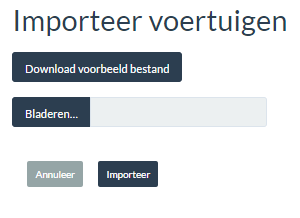
\includegraphics[width=0.5\textwidth]{img/fig25.png}
	\caption{Importeer lijst van voertuigen} 
	\label{fig:25} 
\end{figure}
\newpage
\subsection{Voertuigen}
\label{vehicles}
\subsubsection{Aanmaken}
\begin{todolist}
	\item[\done] Administrator
	\item[\done] Productiebeheerder
	\item[\done] Verzekeringsmakelaar
	\item[\wontfix] Klant 
\end{todolist}
\\
\\
Om een voertuig aan te maken, volgt u onderstaande stappen:
\begin{enumerate}
	\item Om voertuigen te zien, heeft u twee opties:
	\begin{enumerate}
		\item Volg de stappen uit sectie \ref{fleet_show} tot u de informatie van de vloot te zien krijgt zoals weergegeven in Figuur \ref{fig:22}.
		\item Volg de stappen uit sectie \ref{vehicle_search} tot u een lijst van voertuigen te zien krijgt.
	\end{enumerate}
	
	\item Om een voertuig aan te maken, klikt u de knop 'Voertuig aanmaken' aan bovenaan de pagina.
	\item U krijgt nu een formulier te zien zoals in Figuur \ref{fig:26} met als titel 'Voertuig aanmaken'.
	\item Vul het formulier op een correcte manier in en bevestig het aanmaken van een voertuig door de knop 'Voertuig aanmaken' aan te klikken (stap 7) of annuleer het proces via de 'Annuleer' knop (stap 8) .
	\item Indien de door u ingevoerde gegevens niet correct waren, krijgt u een gelijkaardige foutmelding te zien zoals weergegeven in Figuur \ref{fig:6}. Vul de gegevens opnieuw in en verbeter uw fouten.
	\item Indien u het aanmaken van een voertuig bevestigt, komt u opnieuw terecht op de informatiepagina van de vloot. 
	
	\item Indien u het aanmaken van een vloot annuleert, komt u opnieuw terecht op de informatiepagina van de vloot. 
\end{enumerate}
\begin{figure}
	\centering
	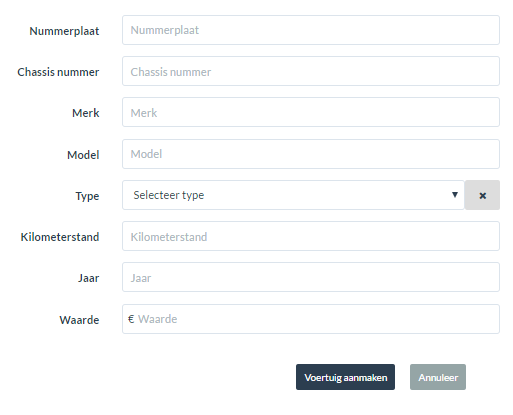
\includegraphics[width=0.8\textwidth]{img/fig26.png}
	\caption{Formulier voertuigen} 
	\label{fig:26} 
\end{figure}



\subsubsection{Bekijken}
\label{vehicle_show}
\begin{todolist}
	\item[\done] Administrator
	\item[\done] Productiebeheerder
	\item[\done] Verzekeringsmakelaar
	\item[\done] Klant 
\end{todolist}
\\
\\
Om een voertuig te bekijken, volgt u onderstaande stappen:
\begin{enumerate}
	\item Om voertuigen te zien, heeft u twee opties:
	\begin{enumerate}
		\item Volg de stappen uit sectie \ref{fleet_show} tot u de informatie van de vloot te zien krijgt zoals weergegeven in Figuur \ref{fig:22}.
		\item Volg de stappen uit sectie \ref{vehicle_search} tot u een lijst van voertuigen te zien krijgt.
	\end{enumerate}
	\item Om een voertuig te bekijken, klikt u het desgewenste voertuig aan	. 
	\item U ziet nu informatie over het gekozen zoals weergegeven in Figuur \ref{fig:27}.
	\item Naast de algemene informatie zie u ook nog de mogelijkheid om de commissies per voertuig te wijzigen en ziet u de verzekering waarvoor het voertuig verzekerd is. Voor verdere informatie cfr. sectie \ref{vehicle_commision} en sectie \ref{vehicle_insurance}.
	\item Tenslotte kan u ook de logs bekijken van het voertuig (cfr. sectie \ref{vehicle_logs})
	\item Indien u wenst terug te keren naar de lijst van vloten, klikt u de knop 'Terug' aan.
\end{enumerate}

\begin{figure}
	\centering
	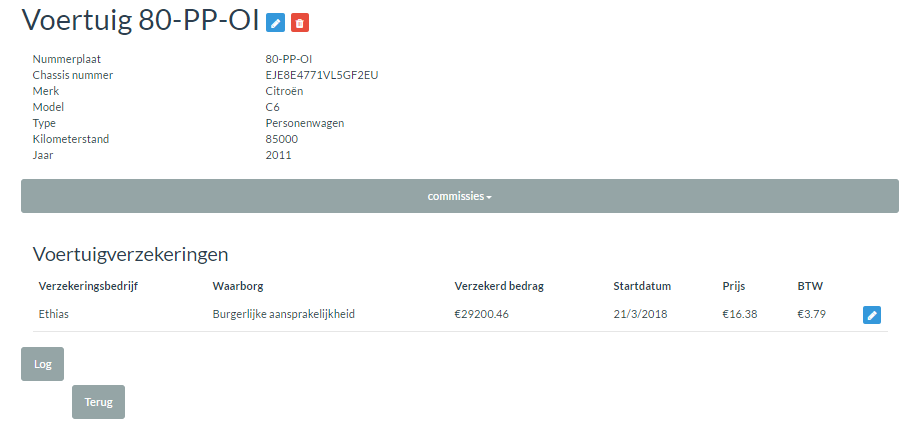
\includegraphics[width=0.8\textwidth]{img/fig27.png}
	\caption{Informatie voertuig} 
	\label{fig:27} 
\end{figure}

\subsubsection{Bewerken}
\begin{todolist}
	\item[\done] Administrator
	\item[\done] Productiebeheerder
	\item[\done] Verzekeringsmakelaar
	\item[\wontfix] Klant 
\end{todolist}
\\
\\
Om een voertuig te bewerken, volgt u onderstaande stappen:
\begin{enumerate}
	\item Om voertuigen te zien, heeft u twee opties:
	\begin{enumerate}
		\item Volg de stappen uit sectie \ref{fleet_show} tot u de informatie van de vloot te zien krijgt zoals weergegeven in Figuur \ref{fig:22}.
		\item Volg de stappen uit sectie \ref{vehicle_search} tot u een lijst van voertuigen te zien krijgt.
	\end{enumerate}
	\item Om een voertuig te bewerken, klikt u het lichtblauwe penseel icoon aan. 
	\item U krijgt nu een formulier te zien zoals in Figuur \ref{fig:26} met als titel 'Voertuig bewerken'.
	\item Vul het formulier op een correcte manier in en bevestig het bewerken van het voertuig door de knop 'Voetuig bewerken' aan te klikken (stap 7) of annuleer het proces via de 'Annuleer' knop (stap 8) .
	\item Indien de door u ingevoerde gegevens niet correct waren, krijgt u een gelijkaardige foutmelding te zien zoals weergegeven in Figuur \ref{fig:6}. Vul de gegevens opnieuw in en verbeter uw fouten.
	\item Indien u het bewerken van een voertuig bevestigt, komt u opnieuw terecht op de informatiepagina van de vloot.  
	\item Indien u het bewerken van een voertuig annuleert, komt u opnieuw terechtop de informatiepagina van de vloot. 
	
\end{enumerate}
\newpage
\subsubsection{Verwijderen}
\begin{todolist}
	\item[\done] Administrator
	\item[\done] Productiebeheerder
	\item[\done] Verzekeringsmakelaar
	\item[\wontfix] Klant 
\end{todolist}
\\
\\
Om een voertuig te verwijderen, volgt u onderstaande stappen:
\begin{enumerate}
	\item Om voertuigen te zien, heeft u twee opties:
	\begin{enumerate}
		\item Volg de stappen uit sectie \ref{fleet_show} tot u de informatie van de vloot te zien krijgt zoals weergegeven in Figuur \ref{fig:22}.
		\item Volg de stappen uit sectie \ref{vehicle_search} tot u een lijst van voertuigen te zien krijgt.
	\end{enumerate}
	\item Om een voertuig te verwijderen, klikt u op het rode vuilbak icoon. 
	\item De applicatie vraagt om een extra bevestiging. Indien u wilt doorgaan met het verwijderen, kiest u voor 'Ja'. In het andere geval kiest u voor 'Nee'.
	\item Het systeem verwijdert het door u gekozen voertuig en u bevindt zich opnieuw naar de informatiepagina van de vloot (Figuur \ref{fig:22}).
\end{enumerate}
\subsubsection{Zoeken in vloot}
\label{vehicle_search}
\begin{todolist}
	\item[\done] Administrator
	\item[\done] Productiebeheerder
	\item[\done] Verzekeringsmakelaar
	\item[\done] Klant 
\end{todolist}
\\
\\
Om een voertuig te zoeken, volgt u onderstaande stappen:
\begin{enumerate}
		\item Volg de stappen uit sectie \ref{fleet_show} tot u de informatie van de vloot te zien krijgt zoals weergegeven in Figuur \ref{fig:22}.
	\item Om een voertuig te zoeken, klikt u de grijze balk met als tekst 'Zoeken' aan. 
	\item Vervolgens krijgt u een formulier te zien zoals weergegeven in Figuur \ref{fig:26}.
	\item Vul de velden in waarop u wilt zoeken en druk op het zoek icoon onderaan het formulier.
	\item U krijgt nu een lijst te zien zoals weergegeven in \ref{fig:22} met alle voertuigen uit uw vloot die voldoen aan uw ingevoerde zoekopdracht.
\end{enumerate}


\subsubsection{Zoeken in alle voertuigen}
\begin{todolist}
	\item[\done] Administrator
	\item[\done] Productiebeheerder
	\item[\done] Verzekeringsmakelaar
	\item[\done] Klant 
\end{todolist}
\\
\\
Om een voertuig te zoeken, volgt u onderstaande stappen:
\begin{enumerate}
		\item Start de Solvas Fleet applicatie en log in. U ziet het startscherm gelijkaardig zoals weergegeven in Figuur \ref{fig:2}.
	\item In de bovenbalk kiest u voor 'Bedrijven' en dan 'Voertuigen'. U ziet nu een lijst van gebruikers zoals weergegeven in Figuur \ref{fig:4}. Indien u als \textit{Klant} actief bent, kiest u voor 'Vloten' en dan 'Voertuigen'.
	\item Om een voertuig te zoeken, klikt u de grijze balk met als tekst 'Zoeken' aan. 
	\item Vervolgens krijgt u een formulier te zien zoals weergegeven in Figuur \ref{fig:26}.
	\item Vul de velden in waarop u wilt zoeken en druk op het zoek icoon onderaan het formulier. Indien u alle velden leeg laat en een zoekaanvraag indient, krijgt u alle voertuigen in het systeem te zien.
	\item U krijgt nu een lijst te zien zoals weergegeven in \ref{fig:29} met alle voertuigen die voldoen aan uw ingevoerde zoekopdracht.
\end{enumerate}


\begin{figure}
	\centering
	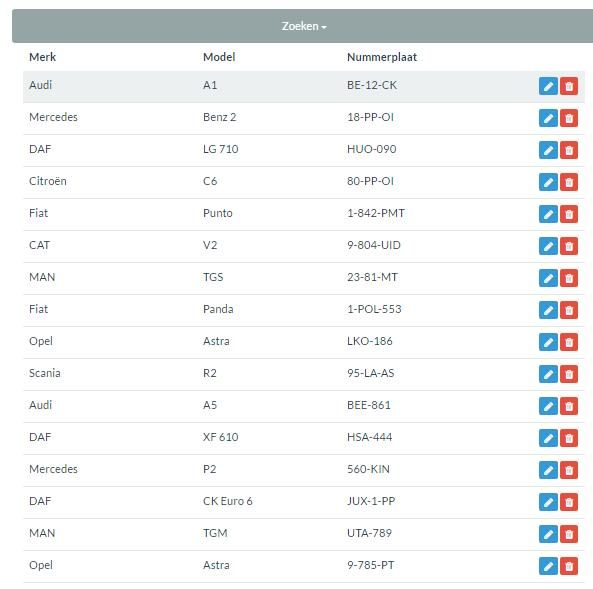
\includegraphics[width=0.5\textwidth]{img/fig29.png}
	\caption{Lijst van voertuigen} 
	\label{fig:29} 
\end{figure}










\subsubsection{Commissie wijzigen}
\begin{todolist}
	\item[\done] Administrator
	\item[\done] Productiebeheerder
	\item[\done] Verzekeringsmakelaar
	\item[\wontfix] Klant 
\end{todolist}
\\
\\
Om de commisies op een voertuig te wijzigen, volgt u onderstaande stappen:
\begin{enumerate}
	\item Volg de stappen uit sectie \ref{vehicle_show} tot u de informatie van het voertuig te zien krijgt zoals weergegeven in Figuur \ref{fig:27}. 
	\item Om de commissies te wijzigen, klikt u de grijze balk met als tekst 'commissies' aan.
	\item Hierop krijgt u de huidige commissiewaarden terug weergegeven zoals in Figuur \ref{fig18}. Indien u deze waarden wil wijzigen dient u de knop 'Wijzig' aan te zetten.
	\item Vervolgens krijgt u een formulier te zien zoals weergegeven in Figuur \ref{fig:18}.
	\item Vul het formulier op een correcte manier in en bevestig het bewerken van de commissies op het voertuig door de knop 'Commissie bewerken' aan te klikken of annuleer het proces via de 'Annuleer' knop.
	\item Indien de door u ingevoerde gegevens niet correct waren, krijgt u een gelijkaardige foutmelding te zien zoals weergegeven in Figuur \ref{fig:6}. Vul de gegevens opnieuw in en verbeter uw fouten.
\end{enumerate}


\

\label{vehicle_commision}
\subsubsection{Logs bekijken}
\label{vehicle_logs}
\begin{todolist}
	\item[\done] Administrator
	\item[\done] Productiebeheerder
	\item[\done] Verzekeringsmakelaar
	\item[\wontfix] Klant 
\end{todolist}
\\
\\
Om de logs van een voertuig te bekijken, volgt u onderstaande stappen:
\begin{enumerate}
	\item  Volg de stappen uit sectie \ref{vehicle_show} tot u de informatie van de vloot te zien krijgt zoals weergegeven in Figuur \ref{fig:27}.
	\item Om de logs te bekijken, klikt u onderdaan de knop 'Log' aan.
	\item U krijgt een lijst van logs te zien van de bewerkingen op dit voertuig zoals weergegeven in Figuur \ref{fig:31}
	\item Indien u wenst terug te keren naar de informatiepagina van de vloot, klikt u de knop 'Terug' aan.
\end{enumerate}

\begin{figure}
	\centering
	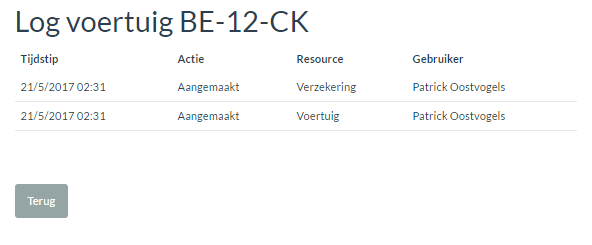
\includegraphics[width=0.5\textwidth]{img/fig31.png}
	\caption{Lijst van logs} 
	\label{fig:31} 
\end{figure}







\newpage
\subsection{Commissies en taksen}
\subsubsection{Per bedrijf}
Voor verdere informatie cfr. sectie \ref{company_commision}.
\subsubsection{Per voertuig}
Voor verdere informatie cfr. sectie \ref{vehicle_commision}.
\subsubsection{Per voertuigtype}
\paragraph{Aanmaken}
\begin{todolist}
	\item[\done] Administrator
	\item[\done] Productiebeheerder
	\item[\done] Verzekeringsmakelaar
	\item[\wontfix] Klant 
\end{todolist}
\\
\\
Om een voertuigtype met bijhorende commissies en taksen aan te maken, volgt u onderstaande stappen:
\begin{enumerate}
	\item Start de Solvas Fleet applicatie en log in. U ziet het startscherm gelijkaardig zoals weergegeven in Figuur \ref{fig:2}.
	\item In de bovenbalk kiest u voor 'Contracten' en dan voor 'Commissies \& taksen'. U ziet nu een lijst van voertuigtypes zoals weergegeven in Figuur \ref{fig:32}.
	\item Om een nieuw voertuigtype aan te maken, klikt u de knop 'Voertuigtype aanmaken' aan bovenaan de pagina.
	\item U krijgt nu een formulier te zien zoals in Figuur \ref{fig:33} met als titel 'Voertuigtype aanmaken'.
	\item Vul het formulier op een correcte manier in en bevestig het aanmaken van een voertuigtype door de knop 'Voertuigtype aanmaken' aan te klikken (stap 7) of annuleer het proces via de 'Annuleer' knop (stap 8) .
	\item Indien de door u ingevoerde gegevens niet correct waren, krijgt u een gelijkaardige foutmelding te zien zoals weergegeven in Figuur \ref{fig:6}. Vul de gegevens opnieuw in en verbeter uw fouten.
	\item Indien u het aanmaken van een voertuigtype bevestigt, komt u opnieuw terecht bij de lijst van voertuigtypes. 
	\item Indien u het aanmaken van een voertuigtype annuleert, komt u opnieuw terecht bij de lijst van voertuigtypes.
	
\end{enumerate}
\begin{figure}
	\centering
	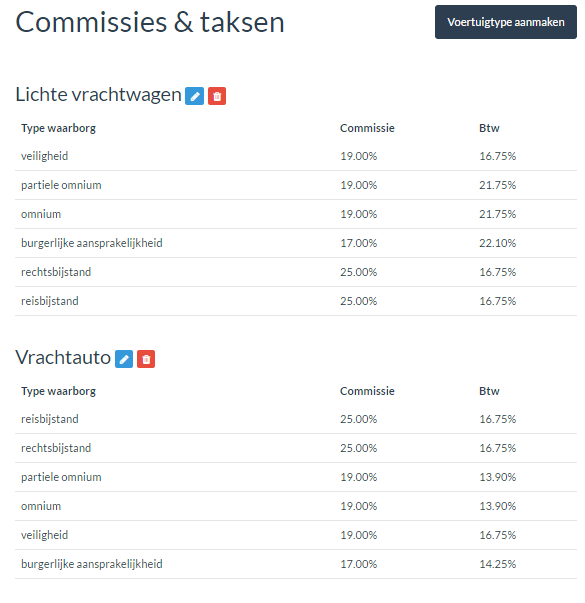
\includegraphics[width=0.6\textwidth]{img/fig32.png}
	\caption{Lijst van voertuigtypes} 
	\label{fig:32} 
\end{figure}
\begin{figure}
	\centering
	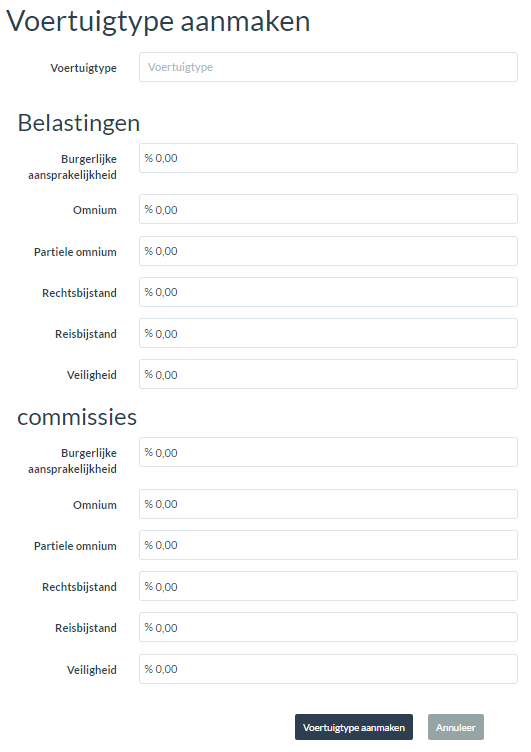
\includegraphics[width=0.6\textwidth]{img/fig33.png}
	\caption{Formulier voertuigtype} 
	\label{fig:33} 
\end{figure}
\newpage
\paragraph{Bekijken}

\begin{todolist}
	\item[\done] Administrator
	\item[\done] Productiebeheerder
	\item[\done] Verzekeringsmakelaar
	\item[\wontfix] Klant 
\end{todolist}
\\
\\
Om een voertuigtype met bijhorende commissies en taksen te bekijken, volgt u onderstaande stappen:
\begin{enumerate}
	\item Start de Solvas Fleet applicatie en log in. U ziet het startscherm gelijkaardig zoals weergegeven in Figuur \ref{fig:2}.
	\item In de bovenbalk kiest u voor 'Contracten' en dan voor 'Commissies \& taksen'. U ziet nu een lijst van voertuigtypes zoals weergegeven in Figuur \ref{fig:32}.
	\item Hier wordt elk voergtuigtype opgelijst en worden de commissie- en takswaarden ook weergegeven per voertuigtype en per verzekeringswaarborg.
	
\end{enumerate}
\newpage
\paragraph{Bewerken}
\begin{todolist}
	\item[\done] Administrator
	\item[\done] Productiebeheerder
	\item[\done] Verzekeringsmakelaar
	\item[\wontfix] Klant 
\end{todolist}
\\
\\
Om een voertuigtype met bijhorende commissies en taksen te bewerken, volgt u onderstaande stappen:
\begin{enumerate}
	\item Start de Solvas Fleet applicatie en log in. U ziet het startscherm gelijkaardig zoals weergegeven in Figuur \ref{fig:2}.
	\item In de bovenbalk kiest u voor 'Contracten' en dan voor 'Commissies \& taksen'. U ziet nu een lijst van voertuigtypes zoals weergegeven in Figuur \ref{fig:32}.
	\item Om een voergtuigtype te bewerken, klikt u het lichtblauwe penseel icoon aan. 
\item U krijgt nu een formulier te zien zoals in Figuur \ref{fig:33} met als titel 'Voergtuigtype bewerken
	\item Vul het formulier op een correcte manier in en bevestig het bewerken van een voertuigtype door de knop 'Voertuigtype bewerken' aan te klikken (stap 7) of annuleer het proces via de 'Annuleer' knop (stap 8) .
	\item Indien de door u ingevoerde gegevens niet correct waren, krijgt u een gelijkaardige foutmelding te zien zoals weergegeven in Figuur \ref{fig:6}. Vul de gegevens opnieuw in en verbeter uw fouten.
	\item Indien u het bewerken van een voertuigtype bevestigt, komt u opnieuw terecht bij de lijst van voertuigtypes. 
	\item Indien u het bewerken van een voertuigtype annuleert, komt u opnieuw terecht bij de lijst van voertuigtypes.
	
\end{enumerate}

\paragraph{Verwijderen}

\begin{todolist}
	\item[\done] Administrator
	\item[\done] Productiebeheerder
	\item[\done] Verzekeringsmakelaar
	\item[\wontfix] Klant 
\end{todolist}
\\
\\
Om een voertuigtype te verwijderen, volgt u onderstaande stappen:
\begin{enumerate}
	\item Start de Solvas Fleet applicatie en log in. U ziet het startscherm gelijkaardig zoals weergegeven in Figuur \ref{fig:2}.
	\item In de bovenbalk kiest u voor 'Contracten' en dan voor 'Commissies \& taksen'. U ziet nu een lijst van voertuigtypes zoals weergegeven in Figuur \ref{fig:32}.
	\item Om een voertuigtype te verwijderen, klikt u op het rode vuilbak icoon. 
	\item De applicatie vraagt om een extra bevestiging. Indien u wilt doorgaan met het verwijderen, kiest u voor 'Ja'. In het andere geval kiest u voor 'Nee'.
	\item Het systeem verwijdert het door u gekozen voertuigtype en u bevindt zich opnieuw naar de informatiepagina over commissies \& taksen (Figuur \ref{fig:32}).
\end{enumerate}




\subsection{Verzekeringen}
\label{insurances}
\subsubsection{Verzekeringscontract}
\label{contract}
\paragraph{Aanmaken}
\begin{todolist}
	\item[\done] Administrator
	\item[\done] Productiebeheerder
	\item[\done] Verzekeringsmakelaar
	\item[\wontfix] Klant 
\end{todolist}
\\
\\
\textbf{Een verzekeringscontract kan ook aangemaakt worden vanuit de homepagina.}
Om een verzekeringscontract aan te maken, volgt u onderstaande stappen:
\begin{enumerate}
	\item Start de Solvas Fleet applicatie en log in. U ziet het startscherm gelijkaardig zoals weergegeven in Figuur \ref{fig:2}.
	\item In de bovenbalk kiest u voor 'Contract'. U ziet nu een lijst van verzekeringscontract zoals weergegeven in Figuur \ref{fig:34}.
	\item Om een verzekeringscontract aan te maken, klikt u de knop 'Contract aanmaken' aan bovenaan de pagina.
	\item U krijgt nu een formulier te zien zoals	 in Figuur \ref{fig:35} met als titel 'Contract aanmaken'.
	\item Vul het formulier op een correcte manier in en bevestig het aanmaken van een verzekeringscontract door de knop 'Contract aanmaken' aan te klikken (stap 7) of annuleer het proces via de 'Annuleer' knop (stap 8) .
	\item Indien de door u ingevoerde gegevens niet correct waren, krijgt u een foutmelding te zien zoals weergegeven in Figuur \ref{fig:6}. Vul de gegevens opnieuw in en verbeter uw fouten.
	\item Indien u het aanmaken van een verzekeringscontract bevestigt, komt u opnieuw terecht bij de lijst van contract.
	\item Indien u het aanmaken van een gebruiker annuleert, komt u opnieuw terecht bij de lijst van gebruikers.
	\item Eenmaal terug bij de lijst van contracten kan u via informatie pagina (cfr. sectie \ref{contract_show}) verzekeringen aan dit contract toevoegen.
\end{enumerate}
\begin{figure}
	\centering
	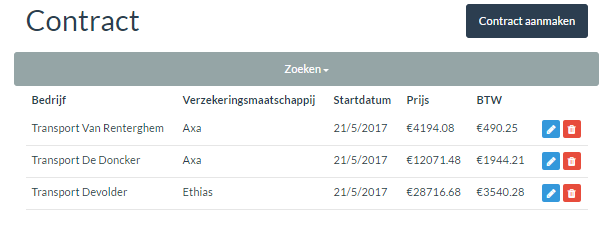
\includegraphics[width=0.8\textwidth]{img/fig34.png}
	\caption{Lijst van verzekeringscontracten} 
	\label{fig:34} 
\end{figure}


\begin{figure}
	\centering
	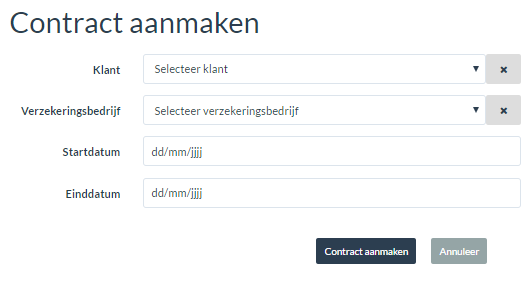
\includegraphics[width=0.5\textwidth]{img/fig35.png}
	\caption{Formulier contract} 
	\label{fig:35} 
\end{figure}

\paragraph{Bekijken}
\label{contract_show}
\begin{todolist}
	\item[\done] Administrator
	\item[\done] Productiebeheerder
	\item[\done] Verzekeringsmakelaar
	\item[\wontfix] Klant 
\end{todolist}
\\
\\
Om een verzekeringscontract te bekijken, volgt u onderstaande stappen:
\begin{enumerate}
	\item Start de Solvas Fleet applicatie en log in. U ziet het startscherm gelijkaardig zoals weergegeven in Figuur \ref{fig:2}.
	\item In de bovenbalk kiest u voor 'Contract'. U ziet nu een lijst van verzekeringscontract zoals weergegeven in Figuur \ref{fig:34}.
	\item Om een verzekeringscontract te bekijken, klikt u het desgewenste verzekeringscontract aan.
	\item U ziet nu informatie over het gekozen verzekeringscontract zoals weergegeven in Figuur \ref{fig:36}. 
	Naast de algemene informatie ziet u ook de verzekeringen die behoren tot dit contract en de verzekeringswaarborgen aangeboden door de verzekeringsmaatschappij. Op beide delen kunnen alle bewerkingen uitgevoerd worden. Voor verdere informatie cfr. sectie \ref{vehicle_insurance} en \ref{sureties}
	\item Indien u wenst terug te keren naar de lijst van gebruikers, klikt u de knop 'Terug' aan..
\end{enumerate}
\begin{figure}
	\centering
	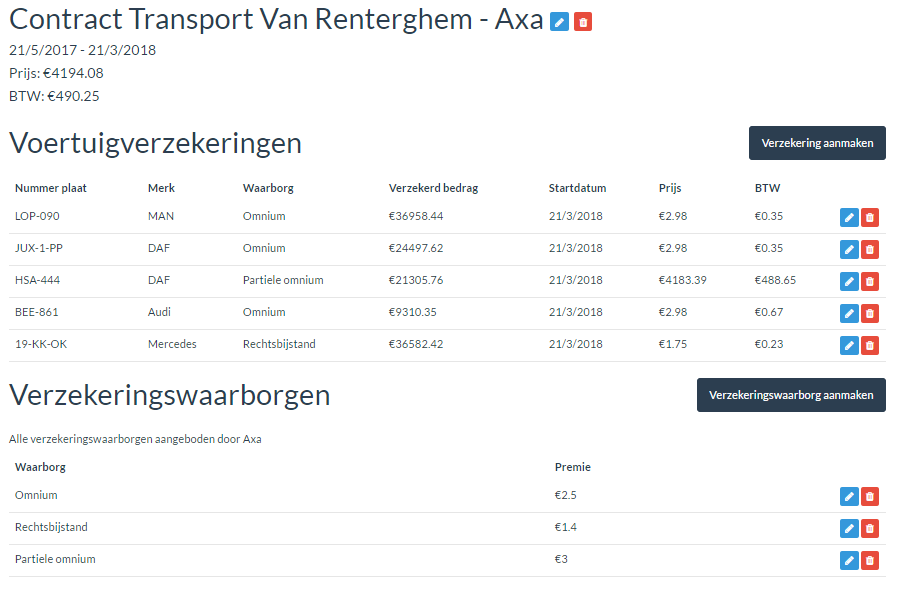
\includegraphics[width=0.8\textwidth]{img/fig36.png}
	\caption{Lijst van verzekeringscontracten} 
	\label{fig:36} 
\end{figure}



\paragraph{Bewerken}
\label{contract_edit}
\begin{todolist}
	\item[\done] Administrator
	\item[\done] Productiebeheerder
	\item[\done] Verzekeringsmakelaar
	\item[\wontfix] Klant 
\end{todolist}
\\
\\
Om een verzekeringscontract te bewerken, volgt u onderstaande stappen:
\begin{enumerate}
	\item Start de Solvas Fleet applicatie en log in. U ziet het startscherm gelijkaardig zoals weergegeven in Figuur \ref{fig:2}.
	\item In de bovenbalk kiest u voor 'Contract'. U ziet nu een lijst van verzekeringscontract zoals weergegeven in Figuur \ref{fig:34}.
	\item Om een verzekeringscontract te bewerken, klikt u het lichtblauwe penseel icoon aan.
	\item U krijgt nu een formulier te zien zoals in Figuur \ref{fig:35} met als titel 'Contract bewerken'.
	\item Vul het formulier op een correcte manier in en bevestig het bewerken van een verzekeringscontract door de knop 'Contract bewerken' aan te klikken (stap 7) of annuleer het proces via de 'Annuleer' knop (stap 8) .
	\item Indien de door u ingevoerde gegevens niet correct waren, krijgt u een foutmelding te zien zoals weergegeven in Figuur \ref{fig:6}. Vul de gegevens opnieuw in en verbeter uw fouten.
	\item Indien u het bewerken van een verzekeringscontract bevestigt, komt u opnieuw terecht bij de lijst van contract.
	\item Indien u het bewerken van een gebruiker annuleert, komt u opnieuw terecht bij de lijst van gebruikers.
\end{enumerate}
\newpage
\paragraph{Verwijderen}
\begin{todolist}
	\item[\done] Administrator
	\item[\done] Productiebeheerder
	\item[\done] Verzekeringsmakelaar
	\item[\wontfix] Klant 
\end{todolist}
\\
\\
\textbf{Het verwijderen van een verzekeringscontract wordt enkel toegestaan indien dit contract geen verzekeringen meer bevat! Voor verdere informatie over het verwijderen van een voertuig verzekering cfr. sectie \ref{vehicle_insurance}}
\\
\\
Om een verzekeringscontract te verwijderen, volgt u onderstaande stappen:
\begin{enumerate}
	\item Start de Solvas Fleet applicatie en log in. U ziet het startscherm weergegeven in Figuur \ref{fig:2}.
	\item In de bovenbalk kiest u voor 'Contract'. U ziet nu een lijst van alle verzekeringscontracten zoals weergegeven in Figuur \ref{fig:34}.
	\item Om een verzekeringscontract te verwijderen, klikt u op het rode vuilbak icoon.
	\item De applicatie vraagt om een extra bevestiging. Indien u wilt doorgaan met het verwijderen, kiest u voor 'Ja'. In het andere geval kiest u voor 'Nee'.
	\item Het systeem verwijdert de door u gekozen gebruiker en u bevindt zich opnieuw naar de lijst van gebruikers (Figuur \ref{fig:4}).
\end{enumerate}

\paragraph{Zoeken}

\begin{todolist}
	\item[\done] Administrator
	\item[\done] Productiebeheerder
	\item[\done] Verzekeringsmakelaar
	\item[\done] Klant 
\end{todolist}
\\
\\
Om een verzekeringscontract te zoeken, volgt u onderstaande stappen:
\begin{enumerate}
	\item Start de Solvas Fleet applicatie en log in. U ziet het startscherm weergegeven in Figuur \ref{fig:2}.
	\item In de bovenbalk kiest u voor 'Contracten'. U ziet nu een lijst van alle contracten zoals weergegeven in Figuur \ref{fig:34}.
	\item Om een contract te zoeken, klikt u de grijze balk met als tekst 'Zoeken' aan. 
	\item Vervolgens krijgt u een formulier te zien zoals weergegeven in Figuur \ref{fig:41}.
	\item Vul de velden in waarop u wilt zoeken en druk op het zoek icoon onderaan het formulier.
	\item U krijgt nu een lijst te zien zoals weergegeven in \ref{fig:34} met alle verzekeringscontract die voldoen aan uw ingevoerde zoekopdracht.
\end{enumerate}

\begin{figure}
	\centering
	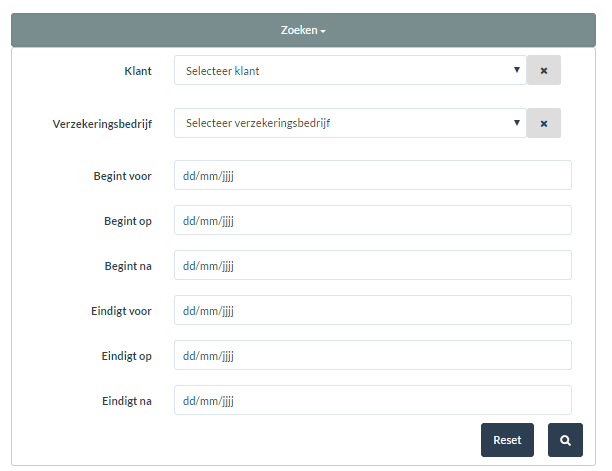
\includegraphics[width=0.5\textwidth]{img/fig41.png}
	\caption{Zoeken naar contract(en)} 
	\label{fig:41} 
\end{figure}
\newpage
\subsubsection{Verzekering}
\label{vehicle_insurance}
\paragraph{Aanmaken}
\begin{todolist}
	\item[\done] Administrator
	\item[\done] Productiebeheerder
	\item[\done] Verzekeringsmakelaar
	\item[\wontfix] Klant 
\end{todolist}
\\
\\
Om een verzekering aan te maken, volgt u onderstaande stappen:
\begin{enumerate}
		\item  Volg de stappen uit sectie \ref{contract_show} tot u de informatie van het contract te zien krijgt zoals weergegeven in Figuur \ref{fig:36}.
	\item Om een verzekering aan te maken en toe te voegen aan het contract, klikt u de knop 'Verzekering aanmaken' aan bovenaan de pagina.
	\item U krijgt nu een formulier te zien zoals in Figuur \ref{fig:37} met als titel 'Verzekering aanmaken'.
	\item Vul het formulier op een correcte manier in en bevestig het aanmaken van een verzekeringscontract door de knop 'Verzekering aanmaken' aan te klikken (stap 7) of annuleer het proces via de 'Annuleer' knop (stap 8) .
	\item Indien de door u ingevoerde gegevens niet correct waren, krijgt u een foutmelding te zien zoals weergegeven in Figuur \ref{fig:6}. Vul de gegevens opnieuw in en verbeter uw fouten.
	\item Indien u het aanmaken van een verzekering bevestigt, komt u opnieuw terecht op de informatiepagina van het contract.
	\item Indien u het aanmaken van een verzekering annuleert, komt u opnieuw terecht op de informatiepagina van het contract.
\end{enumerate}
\begin{figure}
	\centering
	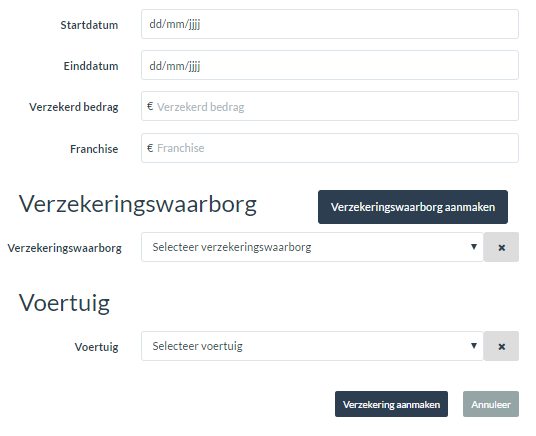
\includegraphics[width=0.8\textwidth]{img/fig37.png}
	\caption{Formulier verzekering} 
	\label{fig:37} 
\end{figure}

\newpage
\paragraph{Bekijken}
\label{vehicle_insurance_show}
\begin{todolist}
	\item[\done] Administrator
	\item[\done] Productiebeheerder
	\item[\done] Verzekeringsmakelaar
	\item[\wontfix] Klant 
\end{todolist}
\\
\\
Om een verzekering te bekijken, volgt u onderstaande stappen:
\begin{enumerate}
		\item  Volg de stappen uit sectie \ref{contract_show} tot u de informatie van het contract te zien krijgt zoals weergegeven in Figuur \ref{fig:36}.
	\item Om een verzekering te bekijken, klikt u de desgewenste verzekering aan.
	\item U ziet nu informatie over de gekozen verzekering zoals weergegeven in Figuur \ref{fig:38}. 
	Naast de algemene informatie ziet u ook het verzekerde voertuig, de bijhorende verzekeringswaarborg en zijn speciale condities en een optie om de groene kaart te generen (cfr: sectie \ref{green_card}). 
\end{enumerate}
\
\begin{figure}
	\centering
	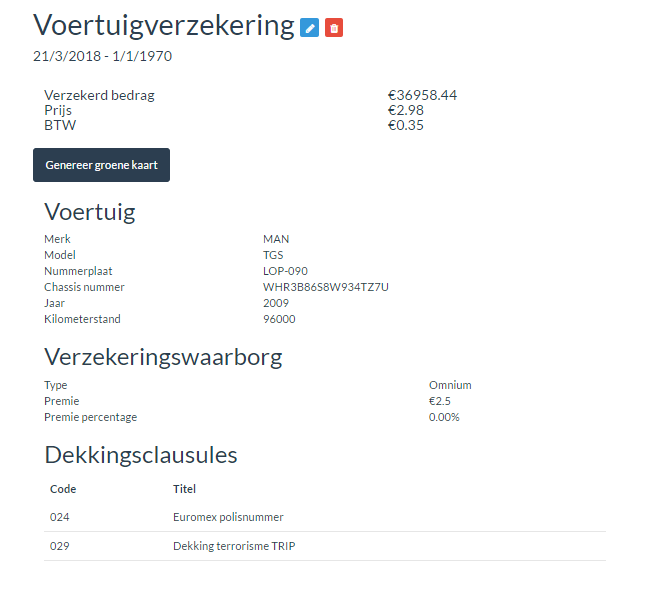
\includegraphics[width=0.5\textwidth]{img/fig38.png}
	\caption{Informatie verzekering} 
	\label{fig:38} 
\end{figure}
\newpage
\paragraph{Bewerken}
\label{insurance_edit}
\begin{todolist}
	\item[\done] Administrator
	\item[\done] Productiebeheerder
	\item[\done] Verzekeringsmakelaar
	\item[\wontfix] Klant 
\end{todolist}
\\
\\
Om een verzekering te bewerken, volgt u onderstaande stappen:
\begin{enumerate}
		\item  Volg de stappen uit sectie \ref{contract_show} tot u de informatie van het contract te zien krijgt zoals weergegeven in Figuur \ref{fig:36}.
	\item Om een verzekering te bewerken, klikt u het lichtblauwe penseel icoon aan.
	\item U krijgt nu een formulier te zien zoals in Figuur \ref{fig:37} met als titel 'Verzekering bewerken'.
	\item Vul het formulier op een correcte manier in en bevestig het bewerken van een verzekering door de knop 'Verzekering bewerken' aan te klikken (stap 7) of annuleer het proces via de 'Annuleer' knop (stap 8) .
	\item Indien de door u ingevoerde gegevens niet correct waren, krijgt u een foutmelding te zien zoals weergegeven in Figuur \ref{fig:6}. Vul de gegevens opnieuw in en verbeter uw fouten.
	\item Indien u het bewerken van een verzekering bevestigt, komt u opnieuw terecht op de informatiepagina van het contract.
	\item Indien u het bewerken van een verzekering annuleert, komt u opnieuw terecht op de informatiepagina van het contract.
\end{enumerate}
\newpage
\paragraph{Verwijderen}
\begin{todolist}
	\item[\done] Administrator
	\item[\done] Productiebeheerder
	\item[\done] Verzekeringsmakelaar
	\item[\wontfix] Klant 
\end{todolist}
\\
\\
Om een verzekering te verwijderen, volgt u onderstaande stappen:
\begin{enumerate}
		\item  Volg de stappen uit sectie \ref{contract_show} tot u de informatie van het contract te zien krijgt zoals weergegeven in Figuur \ref{fig:36}.
	\item Om een verzekering te verwijderen, klikt u op het rode vuilbak icoon.
	\item De applicatie vraagt om een extra bevestiging. Indien u wilt doorgaan met het verwijderen, kiest u voor 'Ja'. In het andere geval kiest u voor 'Nee'.
	\item Het systeem verwijdert de door u gekozen verzekering en u bevindt zich opnieuw naar de informatiepagina van het contract(Figuur \ref{fig:36}).
\end{enumerate}

\subsubsection{Verzekeringswaarborg}
\label{sureties}
\paragraph{Aanmaken}
\begin{todolist}
	\item[\done] Administrator
	\item[\done] Productiebeheerder
	\item[\done] Verzekeringsmakelaar
	\item[\wontfix] Klant 
\end{todolist}
\\
\\
Om een verzekeringswaarborg voor een verzekeringsbedrijf aan te maken, volgt u onderstaande stappen:
\begin{enumerate}
	\item  Volg de stappen uit sectie \ref{contract_show} tot u de informatie van het contract te zien krijgt zoals weergegeven in Figuur \ref{fig:36}.
	\item Om een verzekeringswaarborg voor een verzekeringsbedrijf  aan te maken en toe te voegen aan de aangeboden verzekeringswaarborgen, klikt u de knop 'Verzekeringswaarborg aanmaken' aan bovenaan de pagina.
	\item U krijgt nu een formulier te zien zoals in Figuur \ref{fig:39} met als titel 'Verzekeringswaarborg aanmaken'.
	\item Naast de algemene informatie over de verzekeringswaarborg, is het ook mogelijk om speciale condities toe te voegen aan de verzekeringswaarborg.
	\item Om een speciale conditie toe te voegen aan de verzekeringswaarborg, dient u een speciale conditie te selecteren en vervolgens de knop 'Voeg toe' aan te klikken.
	\item Verder kan u deze speciale conditie opnieuw verwijderen door het rode vuilblak icoon aan te klikken en kan u een nieuwe speciale conditie aanmaken of bestaande bewerken. Voor verdere informatie cfr. sectie \ref{special_conditions}
	\item Vul het formulier op een correcte manier in en bevestig het aanmaken van een verzekeringswaarborg door de knop 'Verzekeringswaarborg aanmaken' aan te klikken (stap 7) of annuleer het proces via de 'Annuleer' knop (stap 8) .
	\item Indien de door u ingevoerde gegevens niet correct waren, krijgt u een foutmelding te zien zoals weergegeven in Figuur \ref{fig:6}. Vul de gegevens opnieuw in en verbeter uw fouten.
	\item Indien u het aanmaken van een verzekeringswaarborg bevestigt, komt u opnieuw terecht bij de lijst van contracten
	\item Indien u het aanmaken van een verzekeringswaarborg annuleert, komt u opnieuw terecht ij de lijst van contracten
\end{enumerate}
\begin{figure}
	\centering
	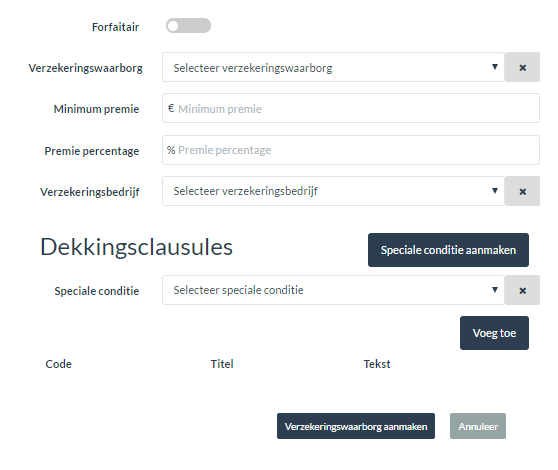
\includegraphics[width=0.8\textwidth]{img/fig39.png}
	\caption{Formulier verzekeringswaarborg} 
	\label{fig:39} 
\end{figure}

\paragraph{Bekijken}
\begin{todolist}
	\item[\done] Administrator
	\item[\done] Productiebeheerder
	\item[\done] Verzekeringsmakelaar
	\item[\wontfix] Klant 
\end{todolist}
\\
\\
Om een verzekeringswaarborg te bekijken, volgt u onderstaande stappen:
\begin{enumerate}
	\item  Volg de stappen uit sectie \ref{contract_show} tot u de informatie van het contract te zien krijgt zoals weergegeven in Figuur \ref{fig:36}.
	\item Om een verzekeringswaarborg te bekijken, klikt u de desgewenste verzekeringswaarborg aan.
	\item U ziet nu informatie over de gekozen verzekeringswaarborg zoals weergegeven in Figuur \ref{fig:40}. 
	Naast de algemene informatie ziet u ook de bijhorende speciale condities die u kan bekijken door aan te klikken (cfr: sectie \ref{special_conditions_show}). 
\end{enumerate}
\
\begin{figure}
	\centering
	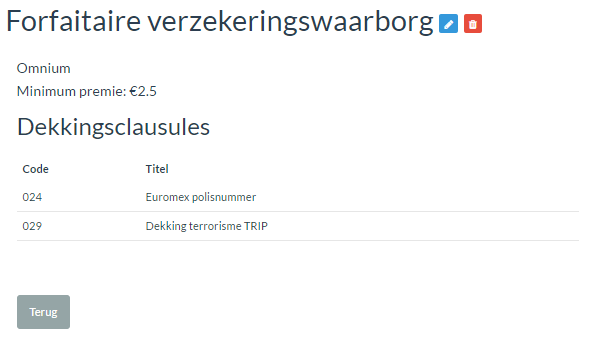
\includegraphics[width=0.5\textwidth]{img/fig40.png}
	\caption{Informatie verzekeringswaarborg} 
	\label{fig:40} 
\end{figure}

\paragraph{Bewerken}
\begin{todolist}
	\item[\done] Administrator
	\item[\done] Productiebeheerder
	\item[\done] Verzekeringsmakelaar
	\item[\wontfix] Klant 
\end{todolist}
\\
\\
Om een verzekeringswaarborg voor een verzekeringsbedrijf te bewerken, volgt u onderstaande stappen:
\begin{enumerate}
	\item  Volg de stappen uit sectie \ref{contract_show} tot u de informatie van het contract te zien krijgt zoals weergegeven in Figuur \ref{fig:36}.
	\item Om een verzekeringswaarborg voor een verzekeringsbedrijf  te bewerken, klikt u het lichtblauwe penseel icoon aan.
	\item U krijgt nu een formulier te zien zoals in Figuur \ref{fig:39} met als titel 'Verzekeringswaarborg aanmaken'.
	\item Naast de algemene informatie over de verzekeringswaarborg, is het ook mogelijk om speciale condities toe te voegen aan de verzekeringswaarborg.
	\item Om een speciale conditie toe te voegen aan de verzekeringswaarborg, dient u een speciale conditie te selecteren en vervolgens de knop 'Voeg toe' aan te klikken.
	\item Verder kan u deze speciale conditie opnieuw verwijderen door het rode vuilblak icoon aan te klikken en kan u een nieuwe speciale conditie aanmaken of bestaande bewerken. Voor verdere informatie cfr. sectie \ref{special_conditions}
	\item Vul het formulier op een correcte manier in en bevestig het bewerken van een verzekeringswaarborg door de knop 'Verzekeringswaarborg aanmaken' aan te klikken (stap 7) of annuleer het proces via de 'Annuleer' knop (stap 8) .
	\item Indien de door u ingevoerde gegevens niet correct waren, krijgt u een foutmelding te zien zoals weergegeven in Figuur \ref{fig:6}. Vul de gegevens opnieuw in en verbeter uw fouten.
	\item Indien u het bewerken van een verzekeringswaarborg bevestigt, komt u opnieuw terecht bij de lijst van contracten
	\item Indien u het bewerken van een verzekeringswaarborg annuleert, komt u opnieuw terecht ij de lijst van contracten
\end{enumerate}

\paragraph{Verwijderen}
\begin{todolist}
	\item[\done] Administrator
	\item[\done] Productiebeheerder
	\item[\done] Verzekeringsmakelaar
	\item[\wontfix] Klant 
\end{todolist}
\\
\\
Om een verzekeringswaarborg te verwijderen, volgt u onderstaande stappen:
\begin{enumerate}
	\item  Volg de stappen uit sectie \ref{contract_show} tot u de informatie van het contract te zien krijgt zoals weergegeven in Figuur \ref{fig:36}.
	\item Om een verzekeringswaarborg te verwijderen, klikt u op het rode vuilbak icoon.
	\item De applicatie vraagt om een extra bevestiging. Indien u wilt doorgaan met het verwijderen, kiest u voor 'Ja'. In het andere geval kiest u voor 'Nee'.
	\item Het systeem verwijdert de door u gekozen verzekeringswaarborg en u bevindt zich opnieuw naar de informatiepagina van het contract(Figuur \ref{fig:36}).
\end{enumerate}












\subsubsection{Speciale condities}
\label{special_conditions}
\paragraph{Aanmaken}
\begin{todolist}
	\item[\done] Administrator
	\item[\done] Productiebeheerder
	\item[\done] Verzekeringsmakelaar
	\item[\wontfix] Klant 
\end{todolist}
\\
\\
Om een speciale conditie aan te maken, volgt u onderstaande stappen:
\begin{enumerate}
	\item Start de Solvas Fleet applicatie en log in. U ziet het startscherm gelijkaardig zoals weergegeven in Figuur \ref{fig:2}.
	\item In de bovenbalk kiest u voor 'Contracten' en dan voor 'Speciale condities'. U ziet nu een lijst van speciale condities zoals weergegeven in Figuur \ref{fig:42}.
	\item Om een speciale conditie aan te maken, klikt u de knop 'Speciale conditie aanmaken' aan bovenaan de pagina. 
	\item U krijgt nu een formulier te zien zoals	 in Figuur \ref{fig:43} met als titel 'Speciale conditie aanmaken'.
	\item Vul het formulier op een correcte manier in en bevestig het aanmaken van een speciale conditie door de knop 'Speciale conditie aanmaken' aan te klikken (stap 7) of annuleer het proces via de 'Annuleer' knop (stap 8) .
	\item Indien de door u ingevoerde gegevens niet correct waren, krijgt u een foutmelding te zien zoals weergegeven in Figuur \ref{fig:6}. Vul de gegevens opnieuw in en verbeter uw fouten.
	\item Indien u het aanmaken van een speciale conditie bevestigt, komt u opnieuw terecht bij de lijst van speciale condities. 
	
	\item Indien u het aanmaken van een speciale conditie annuleert, komt u opnieuw terecht bij de lijst van speciale condities.
	
\end{enumerate}
\begin{figure}
	\centering
	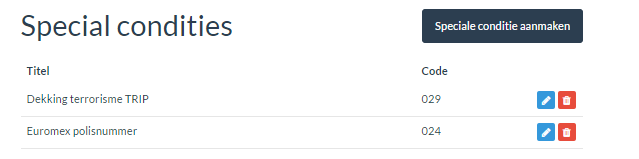
\includegraphics[width=0.8\textwidth]{img/fig42.png}
	\caption{Lijst van speciale condities} 
	\label{fig:42} 
\end{figure}


\begin{figure}
	\centering
	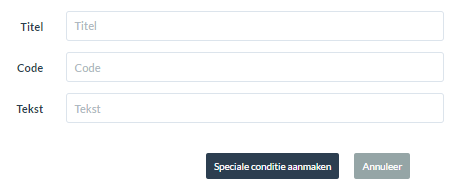
\includegraphics[width=0.5\textwidth]{img/fig43.png}
	\caption{Formulier speciale conditie} 
	\label{fig:43} 
\end{figure}


\paragraph{Bekijken}
\label{special_conditions_show}
\begin{todolist}
	\item[\done] Administrator
	\item[\done] Productiebeheerder
	\item[\done] Verzekeringsmakelaar
	\item[\done] Klant 
\end{todolist}
\\
\\
Om een speciale conditie te bekijken, volgt u onderstaande stappen:
\begin{enumerate}
	\item Start de Solvas Fleet applicatie en log in. U ziet het startscherm gelijkaardig zoals weergegeven in Figuur \ref{fig:2}.
	\item In de bovenbalk kiest u voor 'Contracten' en dan voor 'Speciale condities'. U ziet nu een lijst van speciale condities zoals weergegeven in Figuur \ref{fig:42}. 
	\item Om een speciale conditie te bekijken, klikt u de desgewenste speciale conditie aan. 
	\item U ziet nu informatie over de gekozen speciale conditie zoals weergegeven in Figuur \ref{fig:44}. 
	\item Indien u wenst terug te keren naar de lijst van speciale condities, klikt u de knop 'Terug' aan.
\end{enumerate}

\begin{figure}
	\centering
	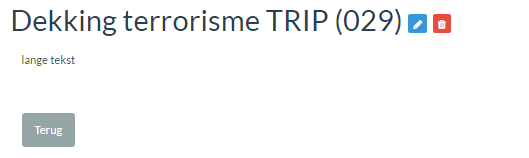
\includegraphics[width=0.8\textwidth]{img/fig44.png}
	\caption{Informatie speciale conditie } 
	\label{fig:44} 
\end{figure}

\paragraph{Bewerken}
\begin{todolist}
	\item[\done] Administrator
	\item[\done] Productiebeheerder
	\item[\done] Verzekeringsmakelaar
	\item[\wontfix] Klant 
\end{todolist}
\\
\\
Om een speciale conditie te bewerken, volgt u onderstaande stappen:
\begin{enumerate}
	\item Start de Solvas Fleet applicatie en log in. U ziet het startscherm gelijkaardig zoals weergegeven in Figuur \ref{fig:2}.
	\item In de bovenbalk kiest u voor 'Contracten' en dan voor 'Speciale condities'. U ziet nu een lijst van speciale condities zoals weergegeven in Figuur \ref{fig:42}.
	\item Om een speciale conditie te bewerken, klikt u het lichtblauwe penseel icoon aan.
	\item U krijgt nu een formulier te zien zoals in Figuur \ref{fig:43} met als titel 'Speciale conditie bewerken'.
	\item Vul het formulier op een correcte manier in en bevestig het bewerken van een speciale conditie door de knop 'Speciale conditie bewerken' aan te klikken (stap 7) of annuleer het proces via de 'Annuleer' knop (stap 8) .
	\item Indien de door u ingevoerde gegevens niet correct waren, krijgt u een foutmelding te zien zoals weergegeven in Figuur \ref{fig:6}. Vul de gegevens opnieuw in en verbeter uw fouten.
	\item Indien u het bewerken van een speciale conditie bevestigt, komt u opnieuw terecht bij de lijst van speciale condities. 
	\item Indien u het bewerken van een speciale conditie annuleert, komt u opnieuw terecht bij de lijst van speciale condities.
	
\end{enumerate}

\paragraph{Verwijderen}

\begin{todolist}
	\item[\done] Administrator
	\item[\done] Productiebeheerder
	\item[\done] Verzekeringsmakelaar
	\item[\wontfix] Klant 
\end{todolist}
\\
\\
Om een speciale conditie te verwijderen, volgt u onderstaande stappen:
\begin{enumerate}
	\item Start de Solvas Fleet applicatie en log in. U ziet het startscherm weergegeven in Figuur \ref{fig:2}.
	\item In de bovenbalk kiest u voor 'Contracten' en dan voor 'Speciale condities'. U ziet nu een lijst van alle speciale condities zoals weergegeven in Figuur \ref{fig:4}.
	\item Om een speciale conditie te verwijderen, klikt u op het rode vuilbak icoon. 
	\item De applicatie vraagt om een extra bevestiging. Indien u wilt doorgaan met het verwijderen, kiest u voor 'Ja'. In het andere geval kiest u voor 'Nee'.
	\item Het systeem verwijdert de door u gekozen speciale conditie en u bevindt zich opnieuw naar de lijst van speciale condities (Figuur \ref{fig:42}).
\end{enumerate}

\subsubsection{Groene Kaart}
\paragraph{Groene kaart genereren}
\label{green_card}
\begin{todolist}
	\item[\done] Administrator
	\item[\done] Productiebeheerder
	\item[\done] Verzekeringsmakelaar
	\item[\wontfix] Klant 
\end{todolist}
\\
\\
Om een groene kaart te genereren, volgt u onderstaande stappen:
\begin{enumerate}
	\item Volg de stappen uit sectie \ref{vehicle_insurance_show} tot u de informatie van de verzekering te zien krijgt zoals weergegeven in Figuur \ref{fig:38}.
	\item Om vervolgens de groene kaart te genereren, klikt u de knop 'Genereer groene kaart' aan zoals weergegeven in Figuur \ref{fig:38}.
	\item Het systeem zal automatisch een groene kaart voor deze verzekering genereren en ervoor zorgen dat uw browser deze automatisch download in PDF-formaat. U kan de gegenereerde groene kaart terug vinden in de ingestelde downloadlocatie van uw browser. De groene kaart ziet er ongeveer uit zoals weergegeven in Figuur \ref{fig:45}
	\item Indien u wenst terug te keren naar de informatiepagina over het contract, klikt u de knop 'Terug' aan.
	
\end{enumerate}
\begin{figure}
	\centering
	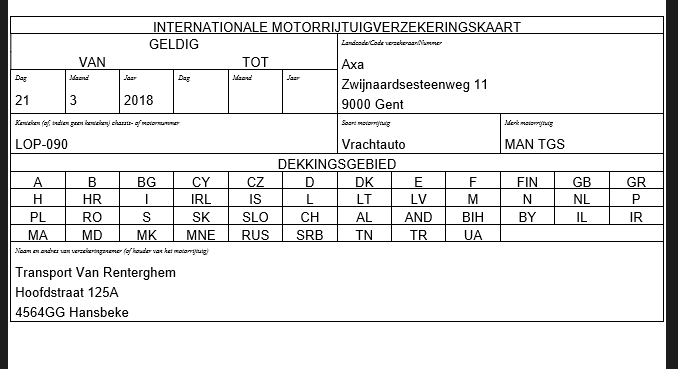
\includegraphics[width=0.8\textwidth]{img/fig45.png}
	\caption{Gegenereerde groene kaart} 
	\label{fig:45} 
\end{figure}



\newpage
\subsection{Facturen}
\subsubsection{Bekijken}
\label{invoice_show}
\begin{todolist}
	\item[\done] Administrator
	\item[\done] Productiebeheerder
	\item[\done] Verzekeringsmakelaar
	\item[\done] Klant 
\end{todolist}
\\
\\
Om een factuur te bekijken, volgt u onderstaande stappen:
\begin{enumerate}
	\item Volg de stappen uit sectie \ref{company_invoice_show} tot u de lijst van facturen van het bedrijf te zien krijgt zoals weergegeven in Figuur \ref{fig:19}.
	\item Om vervolgens een afzonderlijke factuur te bekijken, klikt u de desgewenste factuur aan.
	\item U ziet nu informatie over de gekozen factuur zoals weergegeven in Figuur \ref{fig:46}. 
	\item Indien u wenst terug te keren naar de lijst van facturen, klikt u de knop 'Terug' aan.
	
\end{enumerate}
\begin{figure}
	\centering
	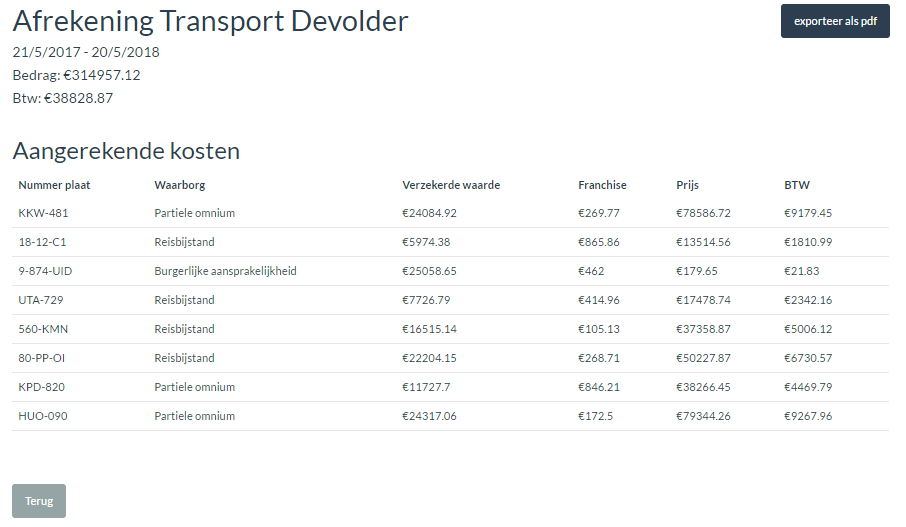
\includegraphics[width=0.8\textwidth]{img/fig46.png}
	\caption{Informatie factuur} 
	\label{fig:46} 
\end{figure}

\newpage
\subsubsection{Exporteer als PDF}
\begin{todolist}
	\item[\done] Administrator
	\item[\done] Productiebeheerder
	\item[\done] Verzekeringsmakelaar
	\item[\done] Klant 
\end{todolist}
\\
\\
Om een factuur als pdf te exporteren, volgt u onderstaande stappen:
\begin{enumerate}
	\item Volg de stappen uit sectie \ref{invoice_show} tot u de informatie van een factuur te zien krijgt zoals weergegeven in Figuur \ref{fig:46}.
	\item Om vervolgens de factuur te exporteren als pdf, klikt u de knop 'exporteer als pdf' aan.
Het systeem zal automatisch een pdf voor deze factuur genereren volgens de ingestelde afrekenings- en facturatieperiode en ervoor zorgen dat uw browser deze automatisch download in PDF-formaat. U kan de gegenereerde pdf terug vinden in de ingestelde downloadlocatie van uw browser. 
\item Indien u wenst terug te keren naar de lijst van facturen, klikt u de knop 'Terug' aan.
	
\end{enumerate}
%\begin{figure}
%	\centering
%	\includegraphics[width=0.8\textwidth]{img/fig48.png}
%	\caption{Factuur in PDF-formaat} 
%	\label{fig:48} 
%\end{figure}

\subsubsection{Instellen afrekeningsperiode \& facturatieperiode}
\begin{todolist}
	\item[\done] Administrator
	\item[\done] Productiebeheerder
	\item[\done] Verzekeringsmakelaar
	\item[\wontfix] Klant 
\end{todolist}
\\
\\
Zowel de afrekenings- als facturatieperiode kunnen ingesteld worden bij het aanmaken en bewerken van een bedrijf.
Voor verdere informatie cfr. sectie \ref{company_new} en sectie \ref{company_edit}.
\end{document}
